\documentclass[journal]{IEEEtran}
\usepackage{amsmath,amsfonts}
\usepackage{algorithmic}
\usepackage{algorithm}
\usepackage{booktabs}
\usepackage{multirow}
\usepackage{siunitx}

\sisetup{
    table-number-alignment = center,
    round-mode = places,
    round-precision = 5
}
\renewcommand{\algorithmicrequire}{\textbf{Input:}}
\renewcommand{\algorithmicensure}{\textbf{Output:}}
\usepackage{array}
\usepackage[caption=false,font=normalsize,labelfont=sf,textfont=sf]{subfig}
\usepackage{textcomp}
\usepackage{stfloats}
\usepackage{url}
\usepackage{verbatim}
\usepackage{graphicx}
\usepackage[compress]{cite}
\hyphenation{op-tical net-works semi-conduc-tor IEEE-Xplore}
% updated with editorial comments 8/9/2021

\begin{document}

\title{Noise-Robust Adaptive Meta-Adversarial Imitation Learning via Confidence-Aware Diffusion Guidance}

\author{IEEE Publication Technology,~\IEEEmembership{Staff,~IEEE,}
        % <-this % stops a space
\thanks{This paper was produced by the IEEE Publication Technology Group. They are in Piscataway, NJ.}% <-this % stops a space
\thanks{Manuscript received April 19, 2021; revised August 16, 2021.}}

% The paper headers
\markboth{Journal of \LaTeX\ Class Files,~Vol.~14, No.~8, August~2021}%
{Shell \MakeLowercase{\textit{et al.}}: A Sample Article Using IEEEtran.cls for IEEE Journals}

% \IEEEpubid{0000--0000/00\$00.00~\copyright~2021 IEEE}
% Remember, if you use this you must call \IEEEpubidadjcol in the second
% column for its text to clear the IEEEpubid mark.

\maketitle

\begin{abstract}
This article proposes a noise-robust adaptive meta-adversarial imitation learning (AMAIL) approach to address key challenges in imitation learning, including training instability, low sample efficiency, and limited robustness under imperfect demonstrations. Specifically, an adaptive meta-learning network (AMLN) is introduced to extract latent behavioral priors from offline expert demonstrations and provide auxiliary guidance for policy optimization. In addition, a diffusion-based confidence estimation mechanism is introduced to adaptively regulate the influence of meta-guided imitation signals, enabling a balanced interaction between imitation learning and reinforcement learning during training.
By incorporating adaptive meta-guided optimization into a diffusion-based adversarial framework, the proposed method captures structural patterns in expert behavior while reducing the computational burden typically associated with diffusion models. 
A dynamic confidence weighting mechanism further enhances robustness by suppressing the influence of noisy or suboptimal demonstrations and by mitigating overfitting. Consequently, the proposed framework improves training stability and data efficiency.
Extensive experiments on Gym MuJoCo and PyBullet demonstrate that the proposed method achieves faster convergence, improved stability, and competitive performance compared with representative baseline methods.
\end{abstract}

\begin{IEEEkeywords}
Adversarial imitation learning, diffusion models, adaptive meta-guided optimization, robust policy learning, robotic control.
\end{IEEEkeywords}



\section{Introduction}
\IEEEPARstart{I}{mitation} learning (IL) has become an effective paradigm for acquiring decision-making policies directly from expert demonstrations\cite{hussein2017imitation,zheng2022imitation}. It has demonstrated strong performance across a wide range of domains, including robotic manipulation, autonomous driving, and game artificial intelligence\cite{wan2024lotus,le2022survey,codevilla2018end,silver2016mastering,9904958}. In contrast to conventional reinforcement learning (RL), which depends on manually designed reward functions, imitation learning enables agents to extract behavioral knowledge directly from expert data. With the rapid advancement of deep neural networks, neural network-based imitation learning has evolved into a central research direction, leading to diverse methods that address challenges in stability, efficiency, and generalization\cite{10078377}.

Among these methods, generative adversarial imitation learning (GAIL)\cite{ho2016generative} is one of the most influential frameworks. By formulating policy learning as a minimax game between a generator and a discriminator, GAIL aligns the occupancy distribution of the learned policy with that of the expert. This approach is supported by a solid theoretical foundation and can handle complex and high-dimensional data without explicit reward design. However, adversarial imitation learning often suffers from training instability caused by gradient vanishing or oscillation\cite{arjovsky2017towards}, which is closely related to the inherent vulnerability of adversarial learning mechanisms\cite{yuan2019adversarial}, low sample efficiency due to extensive interaction with the environment, and limited generalization due to strong reliance on expert trajectories.

To address these limitations, extensive studies in adversarial imitation learning and inverse reinforcement learning have focused on improving stability, sample efficiency, and generalization under unknown rewards or imperfect demonstrations\cite{11232478,finn2016guided,10937085}. Existing approaches can be broadly categorized according to their optimization principles and modeling strategies. Adversarial learning-based approaches extend the minimax formulation to enhance robustness and transferability. These approaches can be divided into two categories. The first category includes methods that directly match expert and policy distributions through adversarial training. The second category consists of adversarial inverse reinforcement learning methods, which recover transferable reward functions from demonstrations to guide subsequent policy optimization. Representative methods include GAIL\cite{ho2016generative}, AIRL\cite{fu2017learning}, GoalGAIL\cite{ding2019goal}, GAIfO\cite{torabi2018generative}, DiffAIL\cite{wang2024diffail}, and RB-GAIL\cite{shi2024ranking}. Although effective, these approaches inherit the intrinsic instability of adversarial optimization. Recent studies further incorporate diffusion-based generative modeling into adversarial imitation learning to enhance distribution modeling capability and robustness\cite{wang2024diffail,chi2025diffusion}.

To mitigate this limitation, occupancy measure-based methods such as ValueDICE\cite{kostrikov2019imitation} and DemoDICE\cite{kim2021demodice} reformulate imitation learning as a convex distribution matching problem over state-action occupancy measures. By converting adversarial objectives into tractable convex optimization problems, these methods remove the minimax structure and improve both training stability and sample efficiency. This formulation is particularly suitable for offline learning and settings with imperfect demonstrations. Building on this perspective, another line of research focuses on implicit reward modeling. Methods such as IQ-Learn\cite{garg2021iq} and SQIL\cite{reddy2019sqil} jointly learn the reward function and policy through soft Q-learning formulations or simplified reward constructions. By avoiding explicit adversarial optimization, these methods achieve improved stability, higher sample efficiency, and simpler implementation, while still enabling effective long-horizon imitation. In parallel, diffusion-based policy learning approaches model action generation as a denoising process, providing improved stability and the ability to capture multimodal expert behaviors\cite{chi2025diffusion,pearce2023imitating,11168119,11165204}.
In addition, demonstration weighted approaches, including 2IWIL\cite{wu2019imitation}, IC-GAIL\cite{wu2019imitation}, and WGAIL\cite{wang2021learning}, introduce confidence-aware mechanisms to reweight demonstration data according to estimated quality. By reducing the influence of suboptimal demonstrations, these methods extend imitation learning to practical scenarios where expert data may be noisy, multimodal, or imperfect, a setting closely related to learning under noisy supervision\cite{song2022learning}. Despite these advances, it remains challenging to balance training stability, sample efficiency, and robustness within a unified framework.

Motivated by these challenges, a noise-robust adaptive meta-adversarial imitation learning (AMAIL) framework is proposed to integrate diffusion-based distribution modeling, adaptive meta-guided optimization, and confidence-aware adaptive regulation. The diffusion discriminator first provides reliable behavior consistency estimation, upon which the AMLN extracts latent behavioral priors from expert demonstrations to guide policy optimization. To prevent unreliable demonstrations from destabilizing training, a confidence-aware weighting mechanism is further introduced to adaptively regulate adaptive meta-guided updates. The main contributions of this article are summarized as follows.

\begin{enumerate}
\item[1)] Adaptive meta-guided optimization is incorporated into adversarial imitation learning by exploiting the discrepancy between twin networks to capture structural patterns in expert behavior from offline data. This design reduces the training overhead typically associated with diffusion models, improves controllability, and increases the efficiency of expert data utilization with only a small increase in computational cost.

\item[2)] A dynamic weighting mechanism is introduced within the adaptive meta-guided optimization process, where discriminator outputs regulate the influence of expert demonstrations. By adaptively suppressing excessive imitation and reducing overfitting to noisy expert data, the proposed approach enhances robustness and stabilizes training in high noise environments.
\end{enumerate}
Moreover, the proposed method is evaluated against representative baselines on both simulation and real-world platforms. Experimental results demonstrate that the proposed method achieves faster convergence, improved stability, and competitive performance across diverse tasks. Sensitivity analysis further indicates that the learning rate of the behavioral cloning network and the weighting coefficient of the adaptive meta-learning twin network significantly influence overall performance.



\section{Related Work}
\subsection{Adversarial Imitation Learning}
Generative adversarial imitation learning (GAIL) alleviates the need for manually designed reward functions in reinforcement learning by employing adversarial training\cite{ho2016generative}. In this framework, imitation learning is formulated as a minimax game between a policy and a discriminator, enabling end-to-end policy optimization through occupancy measure matching between expert and generated trajectories. Building on this foundation, Adversarial Inverse Reinforcement Learning (AIRL)\cite{fu2017learning} introduces a structured reward decomposition from the inverse reinforcement learning perspective, which improves policy generalization under changing environments. GoalGAIL\cite{ding2019goal} further extends this formulation to goal-conditioned settings, enabling multi-goal policy learning without explicit reward design.

Beyond the assumption of ideal expert demonstrations, a large body of work has addressed imitation learning under noisy or imperfect data. For example, 2IWIL\cite{wu2019imitation} incorporates importance weighting to reduce bias caused by suboptimal demonstrations, while IC-GAIL\cite{wu2019imitation} integrates confidence estimation into the adversarial framework. WGAIL\cite{wang2021learning} improves robustness by dynamically reweighting demonstrations to suppress low-quality behaviors. Similarly, RB-GAIL\cite{shi2024ranking} employs ranking-based objectives with multiple weighted discriminators, enabling convergence toward optimal policies even with imperfect data. In addition, GAIfO\cite{torabi2018generative} removes the requirement for action annotations by matching distributions only over state observations, which extends applicability to scenarios where action labels are unavailable. Such settings are closely related to learning under noisy supervision, which has been extensively studied in the literature\cite{song2022learning}.

To further improve stability and sample efficiency, several studies reformulate occupancy distribution matching from alternative optimization perspectives. ValueDICE\cite{kostrikov2019imitation} casts the imitation objective as an off-policy optimisation problem, which significantly improves data efficiency. DemoDICE\cite{kim2021demodice} eliminates the minimax structure by converting adversarial objectives into convex optimization problems, enabling stable offline learning. IQ-Learn\cite{garg2021iq} achieves stable imitation through implicit reward recovery within a soft Q-learning framework, while SQIL\cite{reddy2019sqil} adopts a constant reward formulation to support long-horizon imitation without adversarial training.

Despite these advances, most adversarial imitation learning methods rely on binary classification-based discriminators. Such discriminators often lack sufficient expressive capacity to accurately represent complex and high-dimensional action distributions, leading to coarse reward estimation and suboptimal policy learning. This limitation is related to the inherent instability and vulnerability of adversarial learning mechanisms\cite{yuan2019adversarial,lai2024diffusion}, and motivates the development of more expressive generative structures, such as diffusion-based discriminators\cite{wang2024diffail}, to improve distribution modeling and policy performance.

\subsection{Adaptive Meta-Guided Optimization in Imitation and Reinforcement Learning}
Adaptive meta-guided optimization enables models to adapt efficiently from limited data by learning how to learn. Early approaches such as Model Agnostic Meta Learning(MAML)\cite{finn2017model} perform task level gradient-based optimization, allowing rapid adaptation to new tasks with only a few updates. This paradigm has been systematically studied in neural networks as a general framework for fast adaptation across tasks\cite{hospedales2021meta}. Building on this idea, adaptive meta-guided optimization has been increasingly incorporated into imitation learning to address challenges such as expert heterogeneity, task variability, and inconsistent demonstration quality.

In imitation learning, adaptive meta-guided optimization is often used to automatically adjust learning signals or loss weighting mechanisms, thereby reducing reliance on manual tuning. Several approaches employ meta optimization to learn update strategies for reward functions or discriminators, enabling adaptive adjustment according to training progress or demonstration quality. Compared with fixed heuristic strategies, adaptive meta-guided optimization based methods generally provide stronger generalization across tasks and domains.

However, existing adaptive meta-guided optimization approaches in imitation learning often rely on fixed optimization schemes and lack explicit mechanisms to regulate the influence of adaptive meta-guided updates on policy updates. This limitation reduces robustness in scenarios with highly variable demonstration quality and dynamic training conditions, where uncontrolled meta updates may introduce instability or bias.


\subsection{Diffusion Models for Imitation Learning}
Diffusion models have achieved strong performance in generative modeling by capturing complex data distributions through a progressive denoising process, offering improved stability compared with adversarial learning\cite{ho2020denoising}. More recently, diffusion processes have been introduced into imitation learning to model multimodal expert behavior\cite{finn2017model}.

Unlike adversarial approaches, diffusion-based methods explicitly parameterize the joint state action distribution, thereby avoiding instability associated with minimax optimization. For instance, DiffAIL\cite{wang2024diffail} integrates diffusion modeling into adversarial imitation learning to improve discriminator fidelity through more expressive distribution estimation. Other approaches use diffusion models to generate diverse action samples, which helps mitigate mode collapse in multimodal behavior learning\cite{pearce2023imitating}.

Despite these advantages, diffusion-based imitation learning typically relies on iterative multi-step denoising, which introduces substantial computational cost during both training and inference and limits efficiency in online settings. In addition, these methods often require large-scale expert datasets to ensure stable optimization, reducing effectiveness in low data regimes. Furthermore, most existing approaches primarily focus on reproducing expert trajectories, while robustness under perturbations and generalization across tasks remain insufficiently explored.

From a broader perspective, prior research has advanced imitation learning through adversarial optimization, meta learning, and generative modeling. However, achieving accurate distribution modeling through diffusion processes, meta-learning adaptive regulation  in policy optimization, and robust learning from imperfect demonstrations within a unified framework remains an open challenge.
\begin{figure*}[!hpt]
\centering
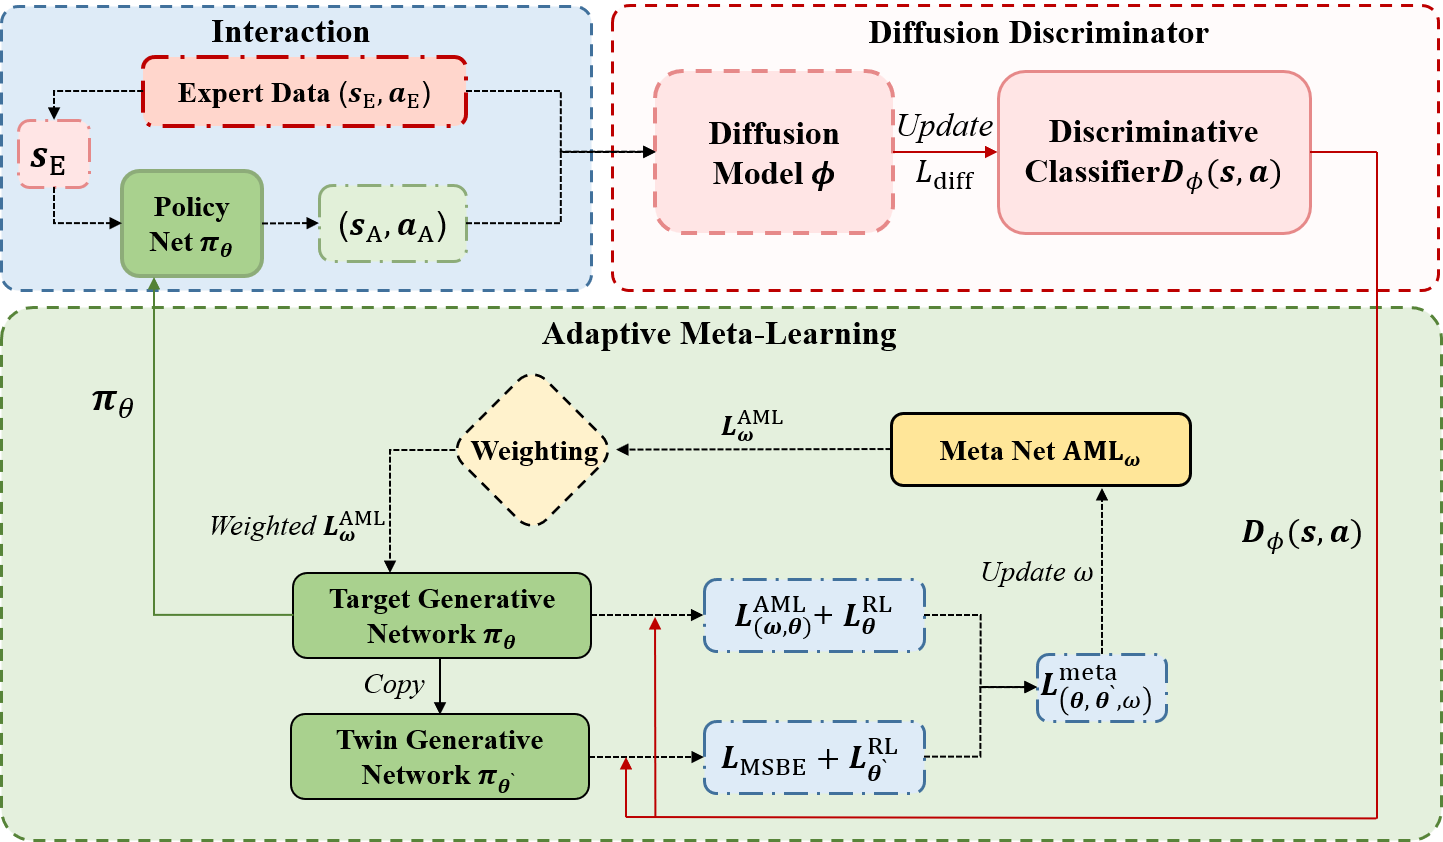
\includegraphics[width=5.5in]{AMLN.png}
\caption{The AMAIL framework consists of three components: policy environment interaction, a diffusion-based discriminator, and an adaptive meta generator. Solid lines denote parameter updates, while dashed lines indicate the flow of input and output data. During training, the generator is updated using a normalized reward provided by the discriminator in the interaction phase. This reward replaces the environment reward during rollout, ensuring that learning is guided by discriminator-based feedback.}
\label{fig_1}
\end{figure*}

\section{Method}
This section presents a noise-robust adaptive meta-adversarial imitation learning (AMAIL) framework, which is designed to improve the training efficiency and stability of diffusion-based adversarial imitation learning\cite{wang2024diffail,lai2024diffusion}. The proposed framework adopts a hierarchical optimization structure inspired by bilevel optimization\cite{finn2017model,deng2025enhancing} in which imitation-guided optimization first extracts structured expert knowledge from offline data and then incorporates this knowledge into online reinforcement learning to guide policy improvement. To further enhance training stability and sample efficiency, an offline data evaluation mechanism is introduced to dynamically regulate the influence of adaptive meta-guided optimization during policy updates\cite{wu2019imitation,song2022learning}.

% The AMAIL framework contains three principal components: policy environment interaction, a diffusion-based discriminator, and an adaptive meta-learning network (AMLN), as illustrated in Fig. \ref{fig_1}. The interaction module generates trajectories and action distributions that are used to train the diffusion discriminator and regulate the meta-learning signal during policy optimization. The diffusion discriminator employs a denoising process to quantify the discrepancy between expert and generated actions by modeling the difference between predicted noise and injected noise, thereby providing more expressive distribution level feedback.

The AMAIL framework forms a hierarchical optimization pipeline consisting of policy-environment interaction, a diffusion-based discriminator, and an adaptive meta-learning network (AMLN), as illustrated in Fig. \ref{fig_1}. During interaction, policy rollouts are first utilized to train the diffusion discriminator, which provides reliable behavior consistency estimation between expert and generated distributions through a denoising process. Based on this distribution-aware feedback, the AMLN further extracts latent behavioral priors from expert demonstrations to guide policy optimization. To improve robustness under noisy demonstrations, adaptive confidence weighting is employed to regulate the influence of meta-guided updates during training.

The AMLN is built upon the distribution-aware feedback provided by the diffusion discriminator and adopts a hierarchical architecture composed of an upper-level meta network and a twin generative network. This design enables the extraction of latent behavioral priors from expert demonstrations, improves data efficiency under limited supervision, and adaptively regulates meta-guided policy optimization. In this work, latent behavioral priors refer to high-level action tendencies and policy adaptation patterns implicitly shared across expert demonstrations.

\subsection{Diffusion Discriminator}
During policy environment interaction, rollouts are collected to train a diffusion-based discriminator and to provide imitation-guided supervision for subsequent policy updates. Unlike conventional binary classifiers, the proposed discriminator derives its decision signal from the denoising process of a diffusion model\cite{ho2020denoising}, where the discrepancy between injected noise and predicted noise reflects the consistency between a state action pair and the target behavior distribution.

Specifically, for a given state-action pair $(s,a)$, a diffusion timestep $t$ is sampled and Gaussian noise $\epsilon$ is injected to construct a corrupted input.
The denoising network $\epsilon_\phi(\cdot)$ then receives $(s,a)$, $t$, and the noisy observation as input, conditioned on a label $\kappa$ that indicates the data source.
The diffusion fitting loss is defined as
\begin{equation}
\label{eq:diff_loss_re}
\mathcal{L}_{\text{diff}}(s,a,\kappa)= \mathbb{E}_{t,\epsilon}\Big[||\epsilon_\phi(s,a,\epsilon,t\mid \kappa)-\epsilon||_2^2\Big]
\end{equation}
where $\kappa$ specifies whether the sample originates from expert demonstrations or agent-generated rollouts. The loss under the expert condition measures alignment with expert behavior, whereas the loss under the agent condition quantifies deviation from the learned policy distribution.

To obtain a stable and bounded learning signal, the diffusion losses are transformed into a discriminative score defined as
\begin{equation}
  \label{eq:discriminator}
  D_\phi(s,a)=\sigma\left(\mathcal{L}_{\text{diff}}(s,a,\kappa_{\text{agent}}) -\mathcal{L}_{\text{diff}}(s,a,\kappa_{\text{expert}})\right)
\end{equation}
where $\sigma(\cdot)$ denotes the sigmoid function. This formulation yields a bounded estimate of expert likeness, where higher values indicate stronger alignment with expert behavior.

The discriminator is optimized using a binary cross-entropy objective, where diffusion losses from expert demonstrations and policy rollouts are used to construct classification targets. Through iterative updates, $D_\phi$ learns to distinguish expert and agent distributions based on denoising discrepancy rather than direct binary classification\cite{wang2024diffail,lai2024diffusion}. Consequently, the resulting output provides a stable and distribution-aware reward signal for downstream policy optimization, thereby alleviating the instability commonly associated with minimax adversarial training.

\subsection{On-Policy Adaptive Meta-Learning Network}

The adaptive meta-learning mechanism is implemented through a dual-layer architecture\cite{finn2017model,hospedales2021meta}. During policy updates, the target policy network $\pi_\theta$ is duplicated to construct a temporary twin network $\pi_{\theta'}$. These two networks correspond to the lower-level learner and the upper-level meta learner, respectively, and are connected through differentiable parameter interactions that facilitate hierarchical adaptive meta-guided optimization.

The lower-level network is optimized using trajectories and rewards collected from environment interactions. To improve learning efficiency, gradient signals from both imitation learning and adaptive meta-guided optimization are incorporated. After independent updates, performance discrepancies arise between the twin network, optimized with reinforcement learning and imitation learning, and the target network, optimized with reinforcement learning and adaptive meta-guided optimization. The upper-level meta network captures this performance gap and uses it as a learning signal for meta optimization. The twin network therefore serves as an imitation-guided reference model, while the target network performs policy optimization under adaptive meta-guidance.

The lower-level optimisation follows the proximal policy optimization framework\cite{schulman2017proximal}. 
Rollout data are first used to compute discounted returns and advantage estimates, followed by multiple epochs of stochastic updates. For each batch, the target network is cloned to form the twin network, which is optimized using a hybrid reinforcement learning and imitation learning objective. The clipped policy loss is defined as
\begin{flalign}
  \label{Agent_loss}
  &\qquad L^{\prime}_{\text{CLIP}}=E[\text{min}(\varDelta_{\ell(\theta)} \cdot A_{\pi}(s,a), \nonumber&\\
  &\quad \quad \quad\quad \quad\quad \quad\text{clip}(\varDelta_{\ell(\theta)},1-\epsilon ,1+\epsilon )\cdot A_{\pi}(s,a))].&
\end{flalign}
where $\varDelta_{\ell(\theta)}$ denotes the probability ratio between the updated and previous policies, and $A_{\pi}(s,a)$ is the corresponding advantage estimate.

To stabilize value estimation, the critic is regularized using a clipped mean-squared error objective
\begin{equation}
\label{Value_loss}
V^{\prime}_{\text{loss}}=\frac{1}{2}\text{max}[(V^{\prime}-r)^2,(V^{\prime}_{\text{clip}}-r)^2]
\end{equation}

Behavior cloning is further incorporated using expert samples within the same batch, yielding the combined twin network objective
\begin{equation}
\label{tmp_loss}
L^{\prime} = L^{\prime}_{a} + c_{\text{v}} \cdot V^{\prime}_{\text{loss}} + c_{\text{bc}} \cdot L^{\text{BC}} - c_{\text{ent}} \cdot \mathbb{E}[H^{\prime}(x_{\theta^{\prime}})]
\end{equation}
where $c_\text{v}$, $c_{\text{bc}}$, and $c_{\text{ent}}$ are weighting coefficients.
This objective is used to update the twin network and serves as the reference baseline for adaptive meta-guided optimization.

The target policy network is then optimized using both reinforcement learning and adaptive meta-guided optimization signals. In addition to the standard policy objective, an adaptive meta-guided optimization loss is introduced as
\begin{equation}
  L^{\text{AML}}_{(\omega,\theta)}=\mathbb{E}[f_{\text{AML}}\cdot W]
\end{equation}
where the initial meta-guided loss is reweighted by the discriminator-derived importance signal $W$\cite{wang2021learning}.


The overall optimization objective becomes
\begin{equation}
\label{actor_loss}
  L = L_{a} + c_{\text{v}} \cdot V_{\text{loss}} + L^{\text{AML}}_{(\omega,\theta)} - c_{\text{ent}} \cdot \mathbb{E}[H(x_{\theta})]
\end{equation}

During the lower-level update, the AMLN receives state-action pairs $(s^d, a^d)$ from demonstrations and the corresponding policy-generated actions $a = \pi_\theta(s^d)$ as inputs. To update the upper level AMLN, the meta objective must remain differentiable with respect to the parameters $\omega$. The upper-level objective is therefore defined as
\begin{equation}
\label{AMLN_loss}
L^{\text{meta}}_{(\theta,\theta^{\prime},\omega)}= \text{tanh}(L_{\pi_{\theta^{\prime}}}-L_{\pi_{\theta}})
\end{equation}
where $L_{\pi_{\theta^{\prime}}}$ and $L_{\pi_{\theta}}$ denote the losses of the twin and target policies, respectively. The AMLN is updated by minimizing the negative of this objective so that configurations in which adaptive meta-guided optimization improves performance are reinforced.
\begin{algorithm}[H]
\caption{Hierarchical Adaptive Meta-Guided Policy Optimization}\label{alg:AML}
\begin{algorithmic}[1]
\REQUIRE Policy network $\pi_\theta$, Discriminator $D_\phi$, AMAIL network $G_\omega$, Expert demonstrations $\mathcal{D}_E$, Rollouts $\mathcal{R}$
\ENSURE Optimized policy network $\pi_{\theta^\star}$, Learned AML network $G_{\omega^\star}$
\STATE \textbf{for} $epoch = 1,2,...,N_{epochs}$ \textbf{do}
\STATE \hspace{0.5cm}Sample mini-batches $\mathcal{B} \sim \mathcal{R} $
\STATE \hspace{0.5cm}\textbf{for} each mini-batch $\mathcal{B}$ \textbf{do}
\STATE \hspace{1cm}Clone policy: $\theta^{\prime}\leftarrow \theta$
\STATE \hspace{1cm}Compute PPO surrogate loss via Eq. \eqref{Agent_loss}
\STATE \hspace{1cm}Compute clipped value loss via Eq. \eqref{Value_loss}
\STATE \hspace{1cm}Sample expert data $(s_E,a_E) \sim \mathcal{D}_E$
\STATE \hspace{1cm}Compute behavior loss $L^{\text{BC}}=\lVert \pi_{\theta^{\prime}}(s_E)-a_E \rVert_2^2$
\STATE \hspace{1cm}Update the twin network using loss $L^{\prime}$ via Eq. \eqref{tmp_loss}
\STATE \hspace{1cm}Evaluate PPO loss using $\pi_{\theta}$
\STATE \hspace{1cm}Generate policy actions $a_\theta=\pi_\theta(s_E)$
\STATE \hspace{1cm}Compute AMLN output $f_{AML}([a_\theta,s_E,a_E])$
\STATE \hspace{1cm}Compute total policy loss via Eq. \eqref{actor_loss}
\STATE \hspace{1cm}Update policy network $\theta$ using loss $L$
\STATE \hspace{1cm}Update AMLN via Eq. \eqref{AMLN_loss}
\STATE \hspace{0.5cm}\textbf{end for}
\STATE \textbf{end for}
\end{algorithmic}
\label{alg1}
\end{algorithm}


\subsection{Adaptive Learning Weights}
Within the proposed architecture, the upper-level AMLN provides an auxiliary optimization signal derived from expert demonstrations. 
This signal guides policy learning by capturing latent structural patterns in expert behavior beyond conventional action matching. The objective is to learn a policy $\pi_\theta(a \mid s)$ that approximates the expert policy $\pi_E(a \mid s)$ from demonstration data. As in standard imitation learning, this formulation remains sensitive to demonstration quality and distributional shift. When demonstrations are noisy or suboptimal, compounding errors may accumulate and lead to substantial performance degradation over long horizons\cite{ross2011reduction,foster2024behavior,vahabpour2024diverse}.

Although moderate demonstration noise may smooth the discriminator decision boundary and produce a regularization effect, excessive noise weakens the ability of the discriminator to identify correct behavioral patterns. This can result in unstable policy updates and directional drift. To address this problem, a confidence-aware adaptive weighting mechanism is introduced to adaptively regulate the contribution of meta-guided optimization signals according to demonstration confidence.

To establish the theoretical basis of this weighting mechanism, the expected discounted return of a policy $\pi$ is defined as
\begin{equation}
\eta (\pi)=\mathbb{E}_{\pi} \left[ \sum_{t=0}^{T} \gamma^t r(s_t,a_t) \right]
\end{equation}

The performance difference between two policies $\widetilde{\pi}$ and $\pi$ can be characterized by $\eta(\widetilde{\pi}) - \eta(\pi)$.
Since directly sampling from $\widetilde{\pi}$ may be impractical\cite{schulman2015trust}, we instead consider the surrogate objective
\begin{equation}
  L^{d_{\pi}}(\widetilde{\pi})=\sum_{s} d_{\pi}(s) \sum_{a} \widetilde{\pi}(a|s) A_{\pi}(s,a)
\end{equation}
where $d_{\pi}(s)=\mathbb{E}[\sum_{t=0}^{T} \gamma^t \mathbf{1}(s_t=s)]$ denotes the discounted state visitation distribution of $\pi$, and $A_\pi(s,a)$ is the advantage function.

To ensure policy improvement while preventing excessive deviation from the reference policy, an $f$ divergence regularization term is introduced over occupancy measures
\begin{equation}
  \max_{\widetilde{\pi}}\quad  L^{d_{\pi}}(\widetilde{\pi}) - \beta D_{f}\!\big(\rho_{\tilde{\pi}}\|\rho_{\pi}\big) ,
	\quad \text{s.t.} \sum_{a}\widetilde{\pi}(a\mid s)=1
\end{equation}
Here, $\beta > 0$ controls the trade-off between performance maximization and distributional proximity to $\pi$. Solving this constrained optimization problem via Lagrangian duality yields

\begin{equation}
  \widetilde{\pi}(a \mid s)=\pi(a \mid s) f_{*}^{\prime}\left(\frac{1}{\beta}\left(A_{\pi}(s, a)+C(s)\right)\right)
\end{equation}
where $f^*$ denotes the convex conjugate of $f$. Under the KL divergence formulation, this leads to the exponential weighting rule
\begin{equation}
  \widetilde{\pi}(a \mid s)=\pi(a \mid s) \exp \left(\frac{1}{\beta}\left(A_{\pi}(s, a)+C(s)\right)\right)
\end{equation}
Consequently, the corresponding occupancy measure satisfies
\begin{equation}
  \rho_{\widetilde{\pi}}(s, a)=\rho_{\pi}(s, a) \exp \left(\frac{1}{\beta}A_{\pi}(s, a)\right)
\end{equation}


Analogous to weighted GAIL (WGAIL)\cite{wang2021learning}, a multiplicative weight function $\omega(s,a)$ is defined such that
\begin{equation}
  \rho_{\widetilde{\pi}}(s, a)= \omega(s, a)\rho_{\pi}(s, a) 
\end{equation}
which establishes a monotonic relationship between $\omega$ and the advantage function $A_\pi$. That is, if the condition $\omega = \text{exp}((1/\beta)A_\pi(s, a))$ is satisfied, the resulting weighting scheme favors actions with larger advantages. Therefore, adaptive weighting is theoretically grounded in advantage based policy improvement.

% In practice, the true advantage function is not directly accessible. To approximate $\omega(s,a)$, the diffusion discriminator is utilized.
% Let $\mathcal{L}_{\text{diff}}(s,a,c)$ denote the diffusion loss under condition $c$, where $c^{+}$ corresponds to expert data and $c^{-}$ corresponds to agent generated data. The discriminator output is defined as

% In practice, the true advantage function is not directly accessible. 
% To approximate $\omega(s,a)$, the diffusion discriminator is utilized. 
% Let $\mathcal{L}_{\text{diff}}(s,a,c)$ denote the diffusion loss under condition $c$, where $c^{+}$ and $c^{-}$ correspond to expert and agent-generated samples, respectively. Since the diffusion discriminator distinguishes expert and policy distributions through denoising discrepancy, its output can be interpreted as a density-ratio estimator similar to that in adversarial imitation learning\cite{ho2016generative,fu2017learning}. The discriminator output is therefore defined as
% \begin{flalign}
% D_{\phi}^{\ast}(s,a)
% &=
% \frac{e^{-\mathcal{L}_{\text{diff}}(s,a,c^+)}}{
% e^{-\mathcal{L}_{\text{diff}}(s,a,c^+)}
% +
% e^{-\mathcal{L}_{\text{diff}}(s,a,c^-)}
% }
% \notag\\
% &=
% \sigma\!\left(
% \mathcal{L}_{\text{diff}}(s,a,c^-)
% -
% \mathcal{L}_{\text{diff}}(s,a,c^+)
% \right)
% \end{flalign}

% Following WGAIL\cite{wang2021learning}, the optimal discriminator can be approximated as
% \begin{equation}
% D_{\phi}^{\ast}(s,a)
% \approx
% \frac{\pi_{\theta}(a\mid s)}
% {
% \pi_{\theta}(a\mid s)
% +
% \omega(s,a)\pi(a\mid s)
% }
% \end{equation}

% Since $\omega(s,a)\propto \exp(A_\pi(s,a))$, we further obtain
% \begin{equation}
% D_{\phi}^{\ast}(s,a)
% \approx
% \frac{\pi_\theta(a \mid s)}
% {
% \pi_\theta(a \mid s)
% +
% \omega(s,a)\exp(A_\pi(s,a))
% }
% \end{equation}

% % \begin{flalign}
% % D_{\phi}^{\ast}(s,a) &= \frac{e^{-\mathcal{L}_{\text{diff}}(s,a,c^+)}}{e^{-\mathcal{L}_{\text{diff}}(s,a,c^+)}+e^{-\mathcal{L}_{\text{diff}}(s,a,c^-)}} \notag\\
% % &= \sigma(\mathcal{L}_{\text{diff}}(s,a,c^-)-\mathcal{L}_{\text{diff}}(s,a,c^+)) \notag\\
% % &= \frac{\pi_{\theta}(a\mid s)}{\pi_{\theta}(a\mid s)+\omega(s,a)\pi(a \mid s)} \notag \\
% % &= \frac{\pi_\theta(a \mid s)}{\pi_\theta(a \mid s)+\omega(s , a)\text{exp}(A_\pi (s,a))}
% % \end{flalign}



% Following the adversarial learning formulation, the discriminator implicitly estimates the log-density ratio between expert and policy distributions\cite{fu2017learning}. It was previously mentioned that the equation $\omega = \text{exp}((1/\beta)A_\pi(s, a))$ holds true. Motivated by the connection between advantage estimation and density ratio modeling, we further approximate the advantage-related weighting term as $A_{\pi}(s, a) = \text{log} \omega(s, a)^\beta$. Based on this relationship, the optimal discriminator can be expressed as
% \begin{equation}
% D_{\phi }^{\ast }(s,a)=\frac{\pi_\theta(a \mid s)}{\pi_\theta(a \mid s)+\omega(s,a)^{(\beta+1)}}
% \end{equation}

% Solving for $\omega(s,a)$ yields
% \begin{equation}
%   \omega(s,a)=\left[\left(\frac{1}{D_\phi ^{\ast }(s,a)}-1\right)\pi_\theta(a \mid s)\right]^{\frac{1}{\beta+1}}
% \end{equation}

% This formulation enables direct computation of adaptive sample weights from the diffusion discriminator output. Consequently, the weighted AML objective reduces the influence of noisy or low confidence demonstrations, thereby mitigating error accumulation and improving robustness under suboptimal expert data and environmental perturbations.

In practice, the true advantage function is not directly accessible.  
To approximate $\omega(s,a)$, the diffusion discriminator is utilized. 

Let $\mathcal{L}_{\text{diff}}(s,a,c)$ denote the diffusion loss under condition $c$, where $c^{+}$ and $c^{-}$ correspond to expert and agent-generated samples, respectively. Since the diffusion discriminator distinguishes expert and policy distributions through denoising discrepancy, its output can be interpreted as a density-ratio estimator similar to adversarial imitation learning \cite{ho2016generative,fu2017learning}. The discriminator output is defined as
\begin{flalign}
D_{\phi}^{\ast}(s,a)
&=
\frac{e^{-\mathcal{L}_{\text{diff}}(s,a,c^+)}}{
e^{-\mathcal{L}_{\text{diff}}(s,a,c^+)}
+
e^{-\mathcal{L}_{\text{diff}}(s,a,c^-)}
}
\notag\\
&=
\sigma\!\left(
\mathcal{L}_{\text{diff}}(s,a,c^-)
-
\mathcal{L}_{\text{diff}}(s,a,c^+)
\right)
\end{flalign}

Following WGAIL \cite{wang2021learning}, the optimal discriminator can be approximated as
\begin{equation}
D_{\phi}^{\ast}(s,a)
\approx
\frac{\pi_{\theta}(a\mid s)}
{
\pi_{\theta}(a\mid s)
+
\omega(s,a)\pi(a\mid s)
}
\end{equation}

Under the advantage-weighted policy formulation, the policy distribution satisfies 
$\pi(a\mid s)\propto \exp(A_\pi(s,a))$. Combined with the previously defined weighting function 
$\omega(s,a)=\exp\!\left((1/\beta) A_\pi(s,a)\right)$,
the discriminator can be further written as
\begin{equation}
D_{\phi}^{\ast}(s,a)
\approx
\frac{\pi_\theta(a \mid s)}
{
\pi_\theta(a \mid s)
+
\omega(s,a)^{\beta+1}
}
\end{equation}

Solving for $\omega(s,a)$ yields
\begin{equation}
\omega(s,a)
=
\left[
\left(
\frac{1}{D_\phi^\ast(s,a)}-1
\right)
\pi_\theta(a\mid s)
\right]^{\frac{1}{\beta+1}}
\end{equation}

This formulation enables direct computation of adaptive sample weights from the diffusion discriminator output. Consequently, the weighted AML objective suppresses noisy or low-confidence demonstrations, thereby mitigating error accumulation and improving robustness under suboptimal expert data and environmental perturbations.
\begin{figure*}[!t]
\centering

\subfloat[FETCHPUSH]{%
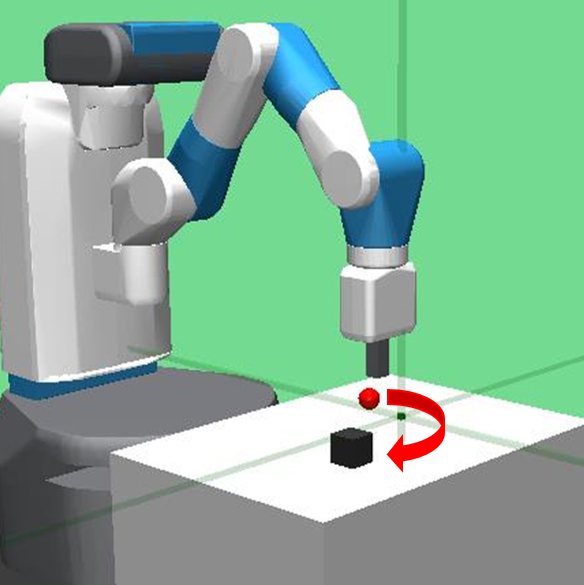
\includegraphics[width=0.16\textwidth]{pic1}%
\label{fig_first_case}}%
\hfill
\subfloat[FETCHPICK]{%
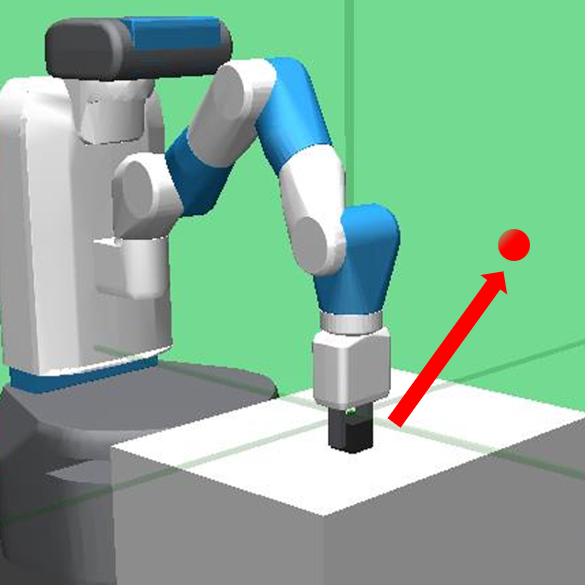
\includegraphics[width=0.16\textwidth]{pic2}%
\label{fig_second_case}}%
\hfill
\subfloat[ANTREACH]{%
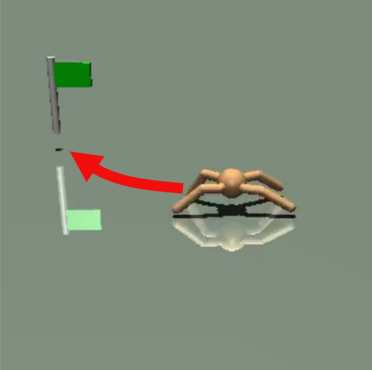
\includegraphics[width=0.16\textwidth]{pic3}%
\label{fig_third_case}}%
\hfill
\subfloat[HANDROTATE]{%
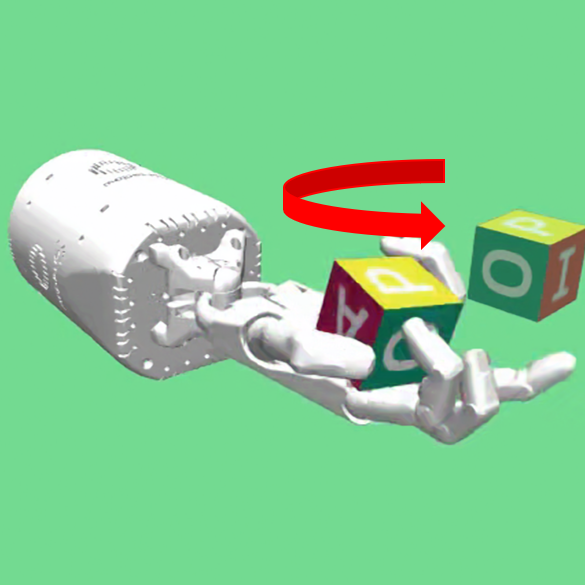
\includegraphics[width=0.16\textwidth]{pic4}%
\label{fig_fourth_case}}%
\hfill
\subfloat[MAZE]{%
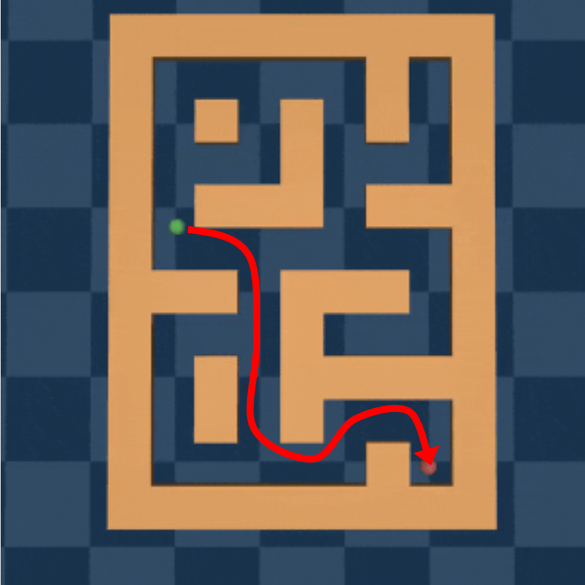
\includegraphics[width=0.16\textwidth]{pic5}%
\label{fig_fifth_case}}%
\hfill
\subfloat[WALKER]{%
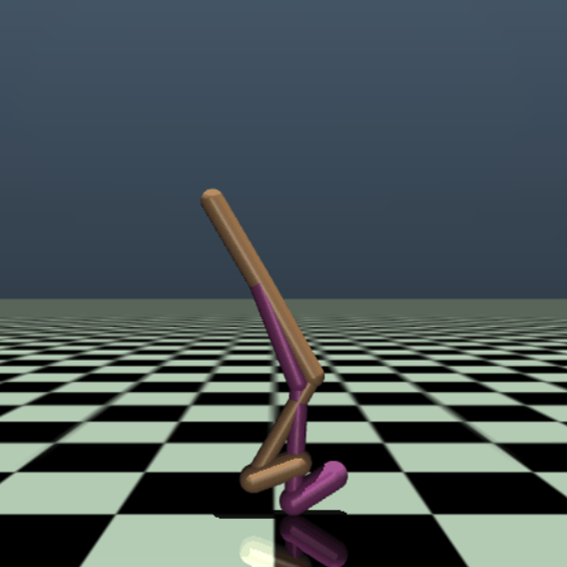
\includegraphics[width=0.16\textwidth]{pic6}%
\label{fig_sixth_case}}%

\caption{The experiments mainly consist of five goal-oriented tasks and one performance-oriented task. (a) The robotic arm needs to push the object to the target point. (b) The robotic arm needs to pick up the object and move it to the target point. (c) The ant agent needs to move to the target point indicated by the flag. (d) The dexterous hand needs to rotate the cube in its hand to the target direction. (e) The agent needs to pass through the maze from the green starting point to reach the red target point. (f) The bipedal walker needs to move forward as far as possible within a fixed time.}
\label{fig_sim}
\end{figure*}


\section{Experiment}

This section evaluates the performance and data efficiency of the proposed AMAIL framework. The objective is to demonstrate its effectiveness in complex environments, as well as its advantages in training efficiency, stability, and generalization compared with existing methods. The proposed approach is evaluated on a set of continuous control tasks, including navigation, robotic manipulation, and locomotion, all implemented on the MuJoCo platform.

\subsection{Simulation setup}
This subsection describes the benchmark environments, task configurations, and expert datasets used for evaluation.

\textbf{FETCHPUSH.} The first evaluation is conducted on the 7 DoF FetchPush manipulation task, as shown in Fig. \ref{fig_first_case}, where a robotic arm is required to push a block to a target location. The 16-dimensional observation vector includes the gripper pose, object pose, relative position, and goal location. Both the initial object state and the target position are randomized across episodes. The expert dataset contains 20311 transitions collected from 664 trajectories\cite{lee2021generalizable}. To evaluate robustness, Gaussian noise is injected into the initial and goal states during training.

\textbf{FETCHPICK.} In the FetchPick task, as shown in Fig. \ref{fig_second_case}, the agent must grasp a block and lift it to a designated target location in 3D space. The observation structure is identical to that of FetchPush. We utilize a dataset containing 50,000 transitions generated by a scripted expert policy\cite{lee2021generalizable}. As in FetchPush, additional noise is applied to the initial and target block positions during training to evaluate noise tolerance and generalization capability.



\textbf{ANTREACH.} As shown in Fig. \ref{fig_third_case}, this task evaluates performance in a high dimensional locomotion setting. A quadruped agent must reach a randomly generated target located along a semicircular boundary. The 132 dimensional state includes joint angles, velocities, contact forces, and relative goal information. The dataset contains 1000 expert trajectories\cite{lee2021generalizable}. Random disturbances are introduced during training to evaluate robustness.

\textbf{HANDROTATE.} As shown in Fig. \ref{fig_fourth_case}, this task involves dexterous manipulation using a Shadow hand with 24 degrees of freedom. The objective is to rotate an object to match a target orientation. The state space is 68 dimensional, and the action space is continuous with 20 dimensions. The expert dataset consists of approximately 10000 transitions collected from 515 trajectories\cite{lee2021generalizable}.

\textbf{MAZE.} In this navigation task, as shown in Fig. \ref{fig_fifth_case}, a point mass agent moves from a random initial position to a fixed goal. Observations include position and velocity, and actions correspond to continuous velocity commands. The dataset includes 100 demonstration trajectories with 18525 transitions\cite{lee2021generalizable}.

\textbf{WALKER.} As shown in Fig. \ref{fig_sixth_case}, this task evaluates locomotion control for a planar bipedal agent. The 17-dimensional state includes joint configurations and velocities, while the 6-dimensional action controls joint torques. The dataset consists of 1000 trajectories\cite{lee2021generalizable}, and random perturbations are introduced during training.



\begin{figure*}[!t]
\centering

\subfloat[FETCHPUSH]{%
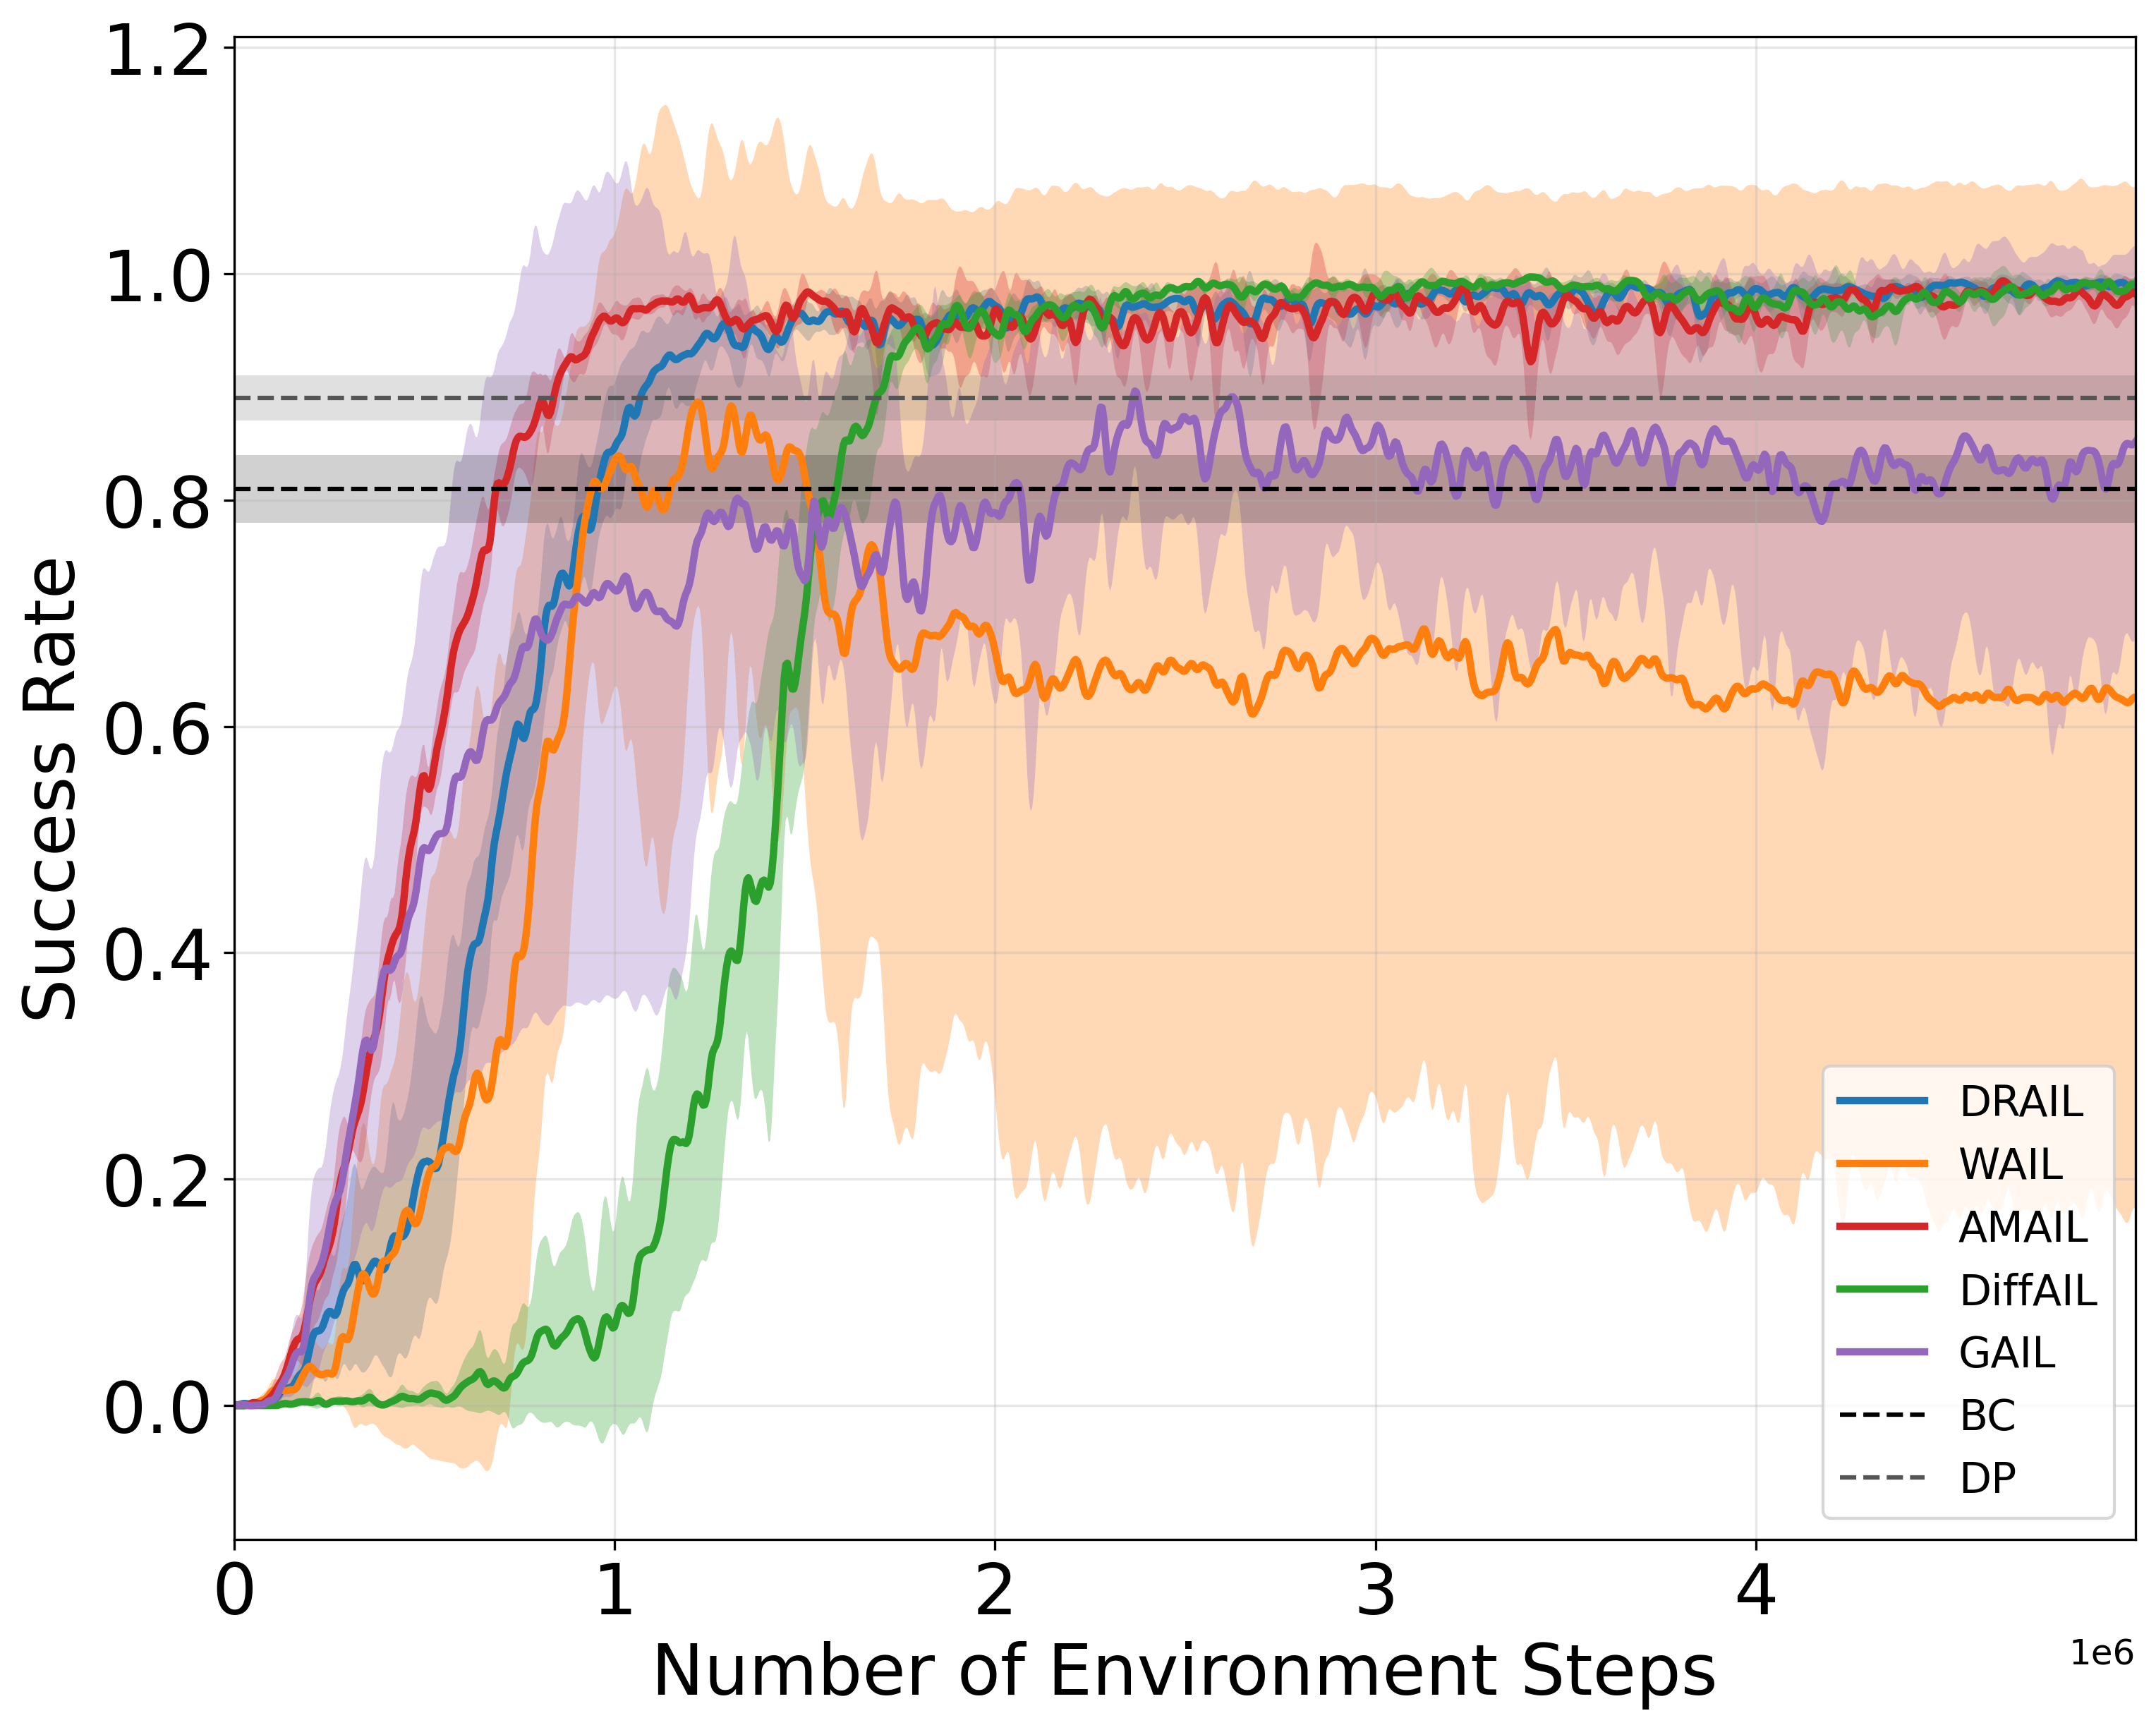
\includegraphics[width=0.33\textwidth]{fetchpush.png}%
\label{fetchpush}}%
\hfill
\subfloat[FETCHPICK]{%
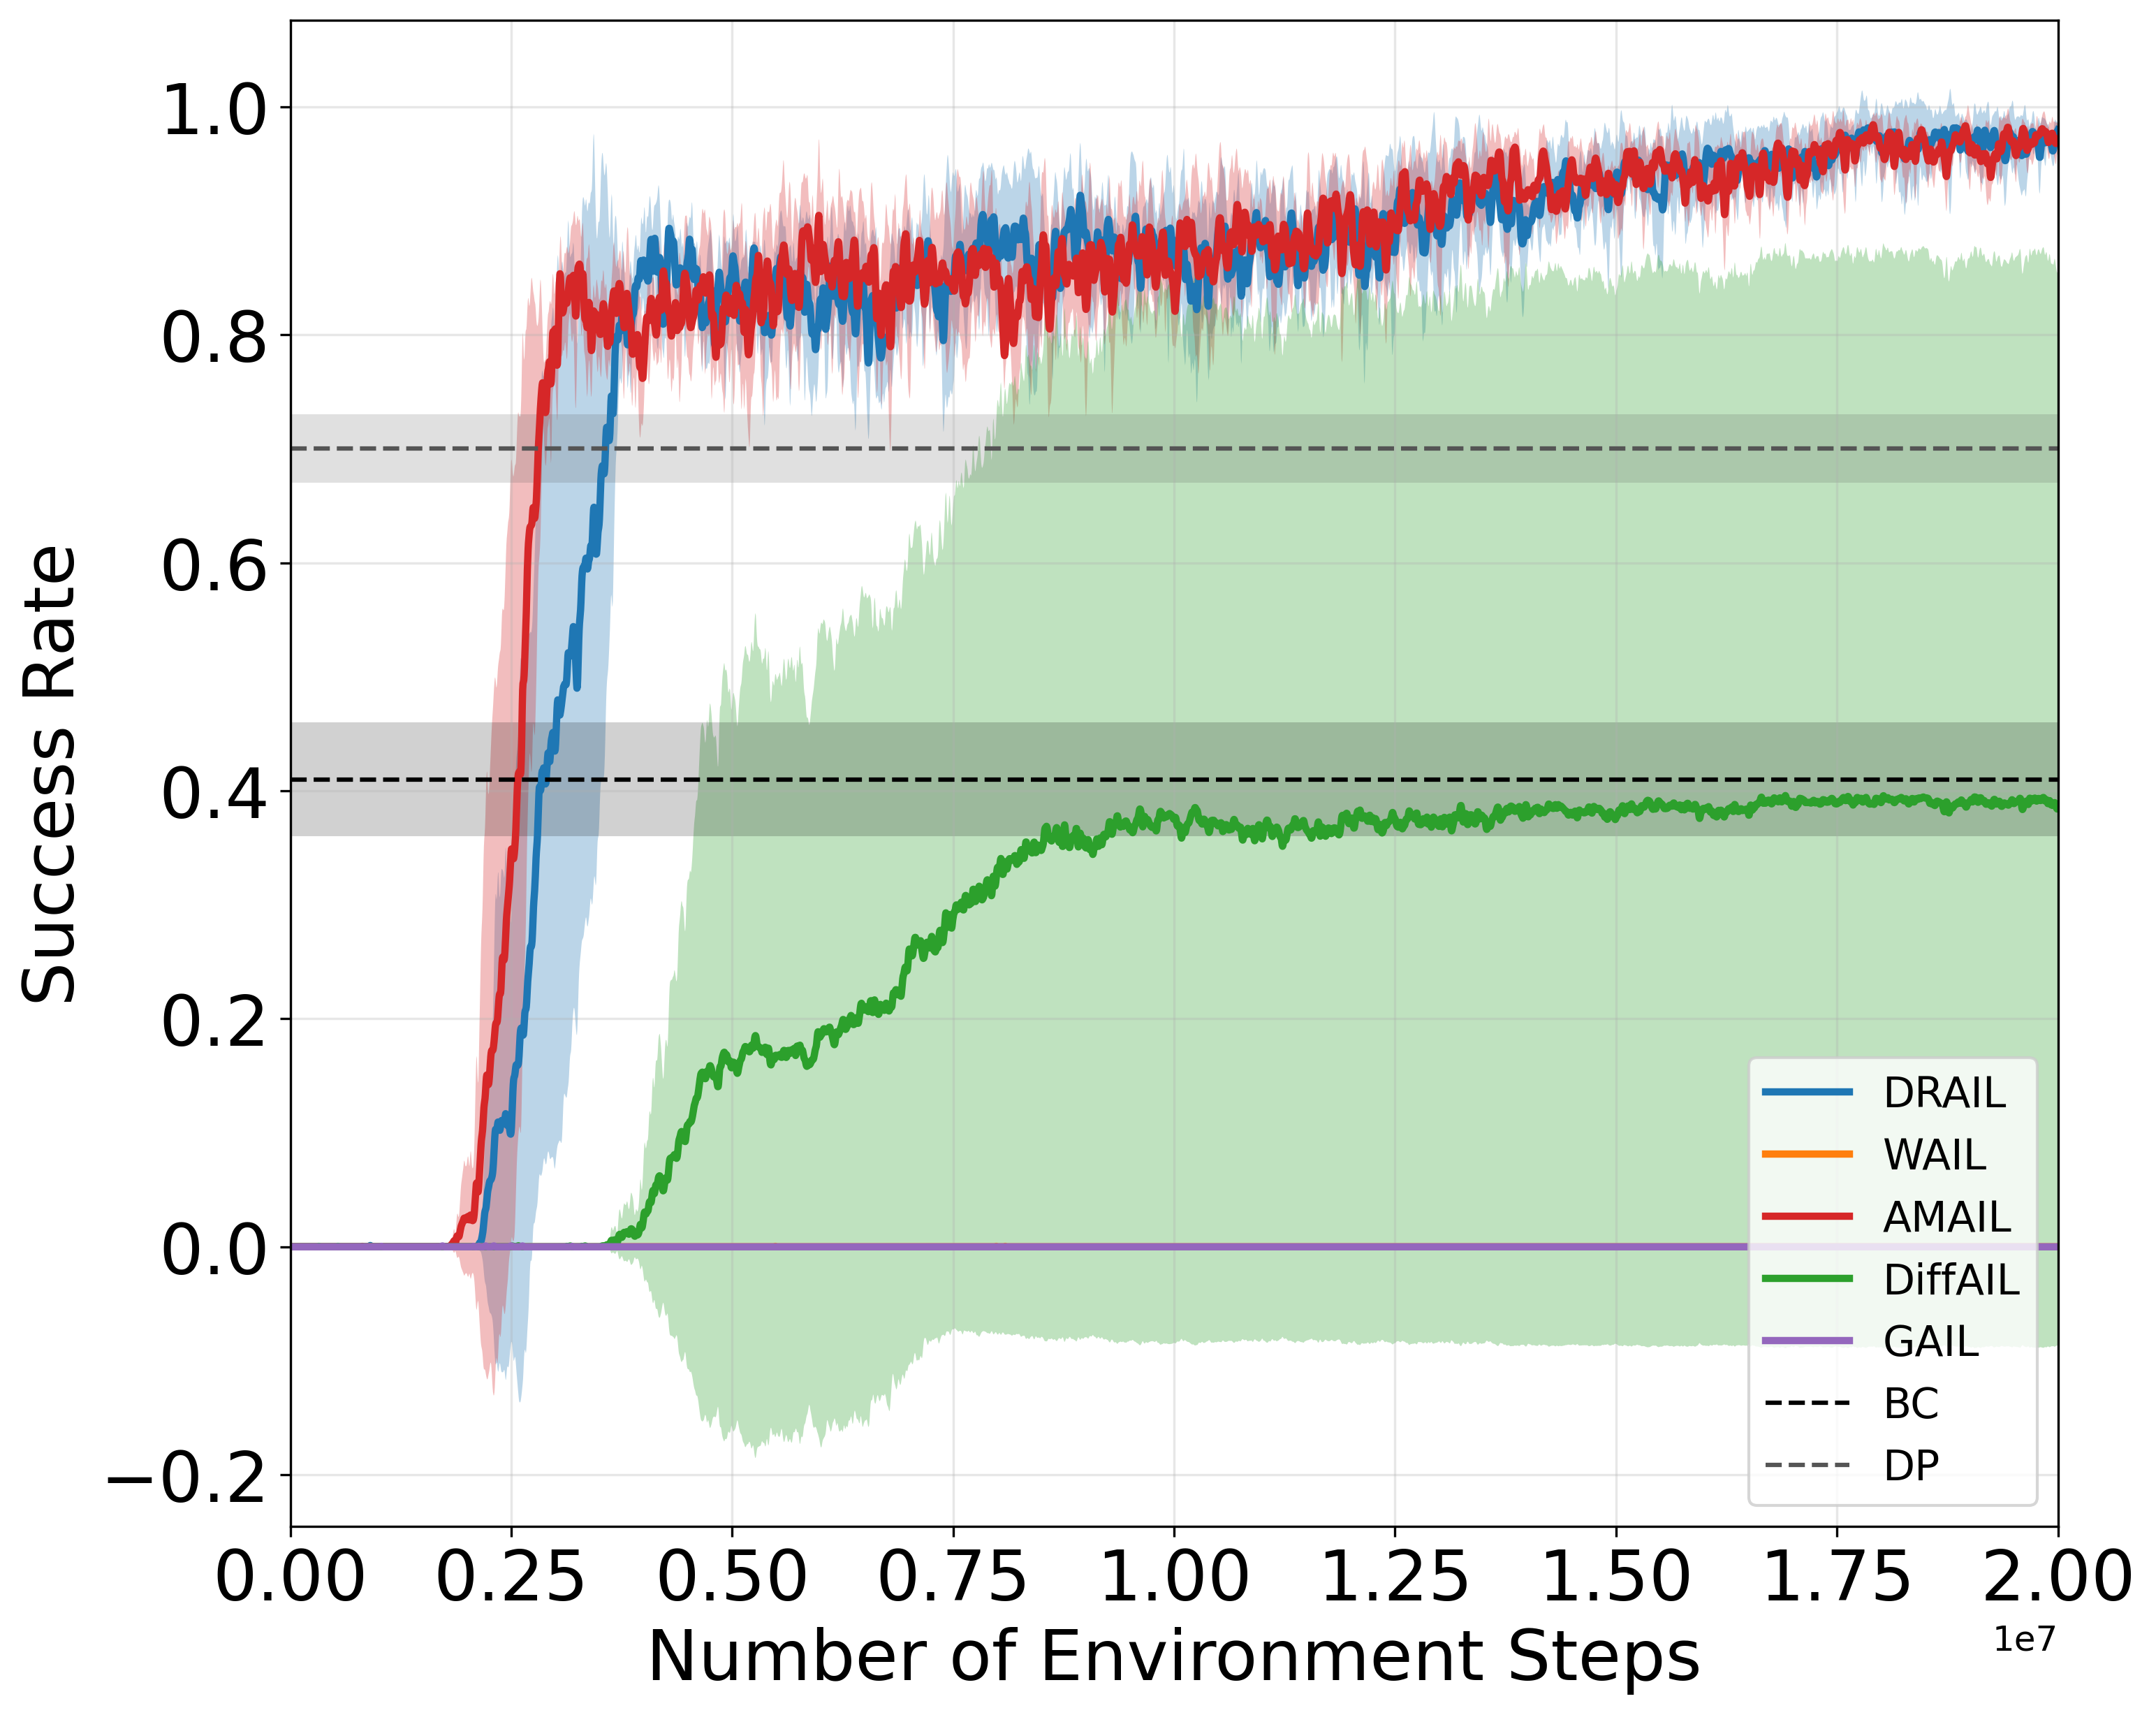
\includegraphics[width=0.33\textwidth]{fetchpick.png}%
\label{fetchpick}}%
\hfill
\subfloat[ANTREACH]{%
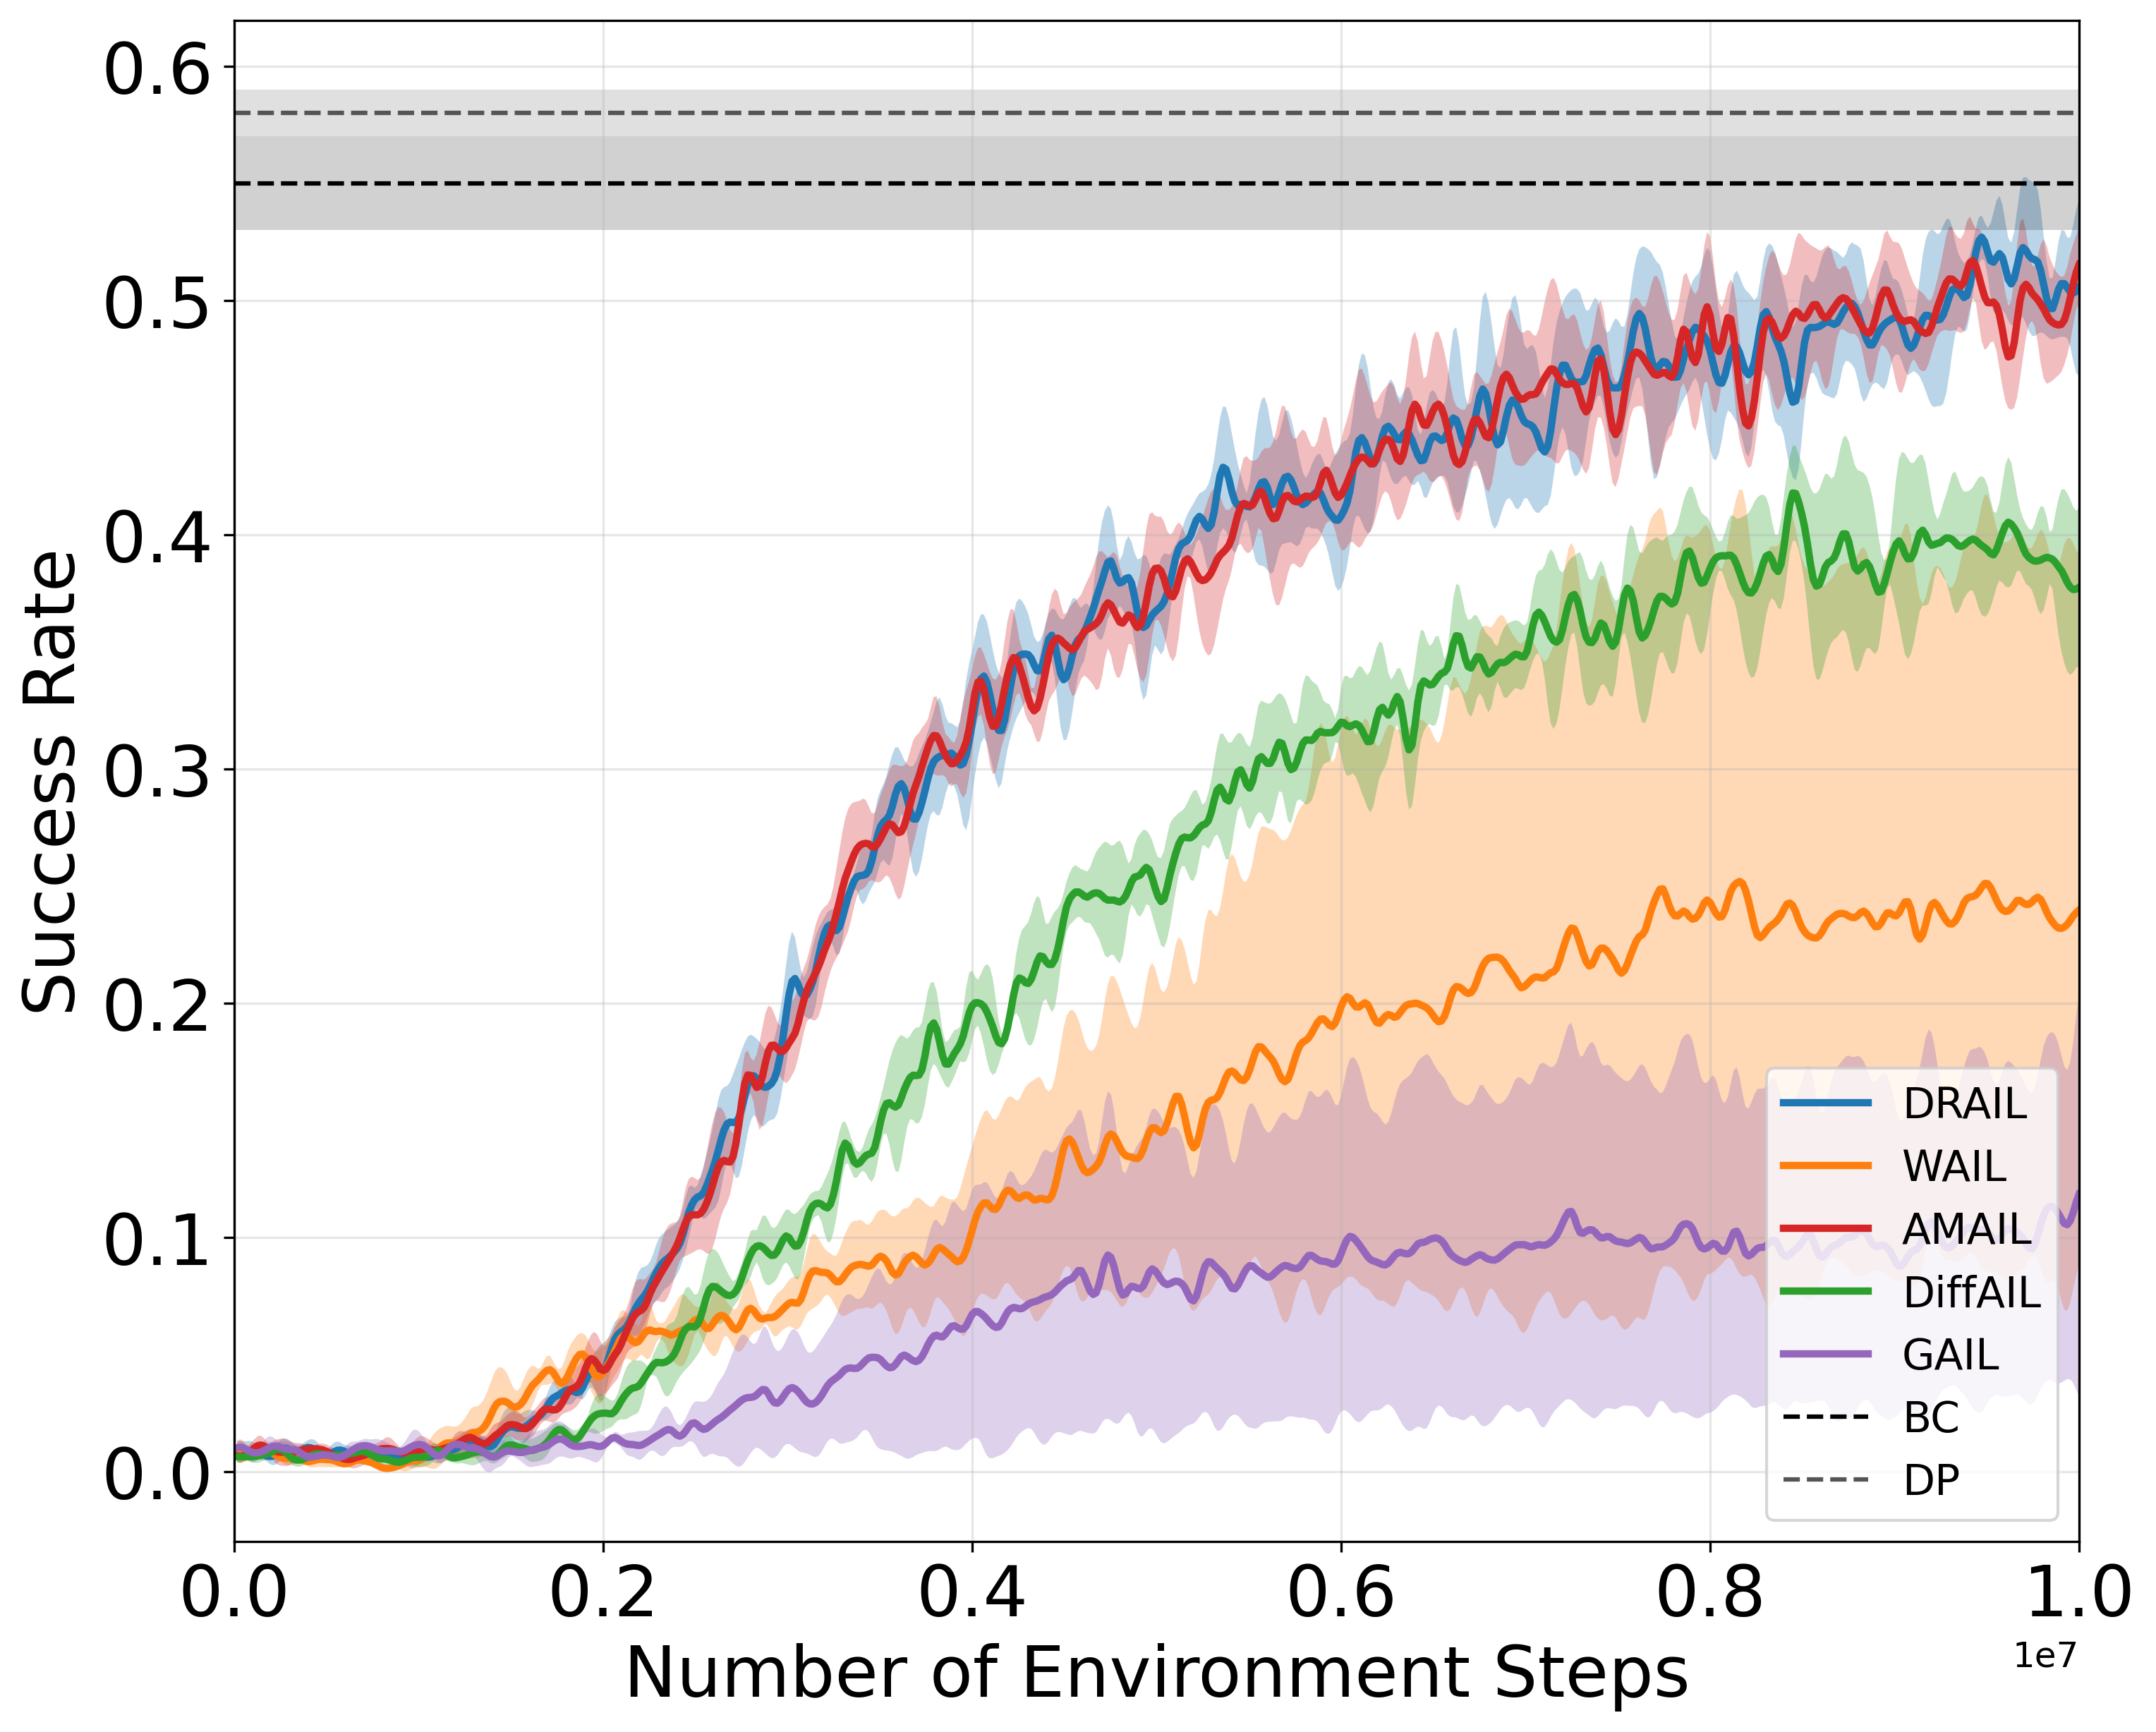
\includegraphics[width=0.33\textwidth]{Antgoal.png}%
\label{antreach}}%
\hfill
\subfloat[HANDROTATE]{%
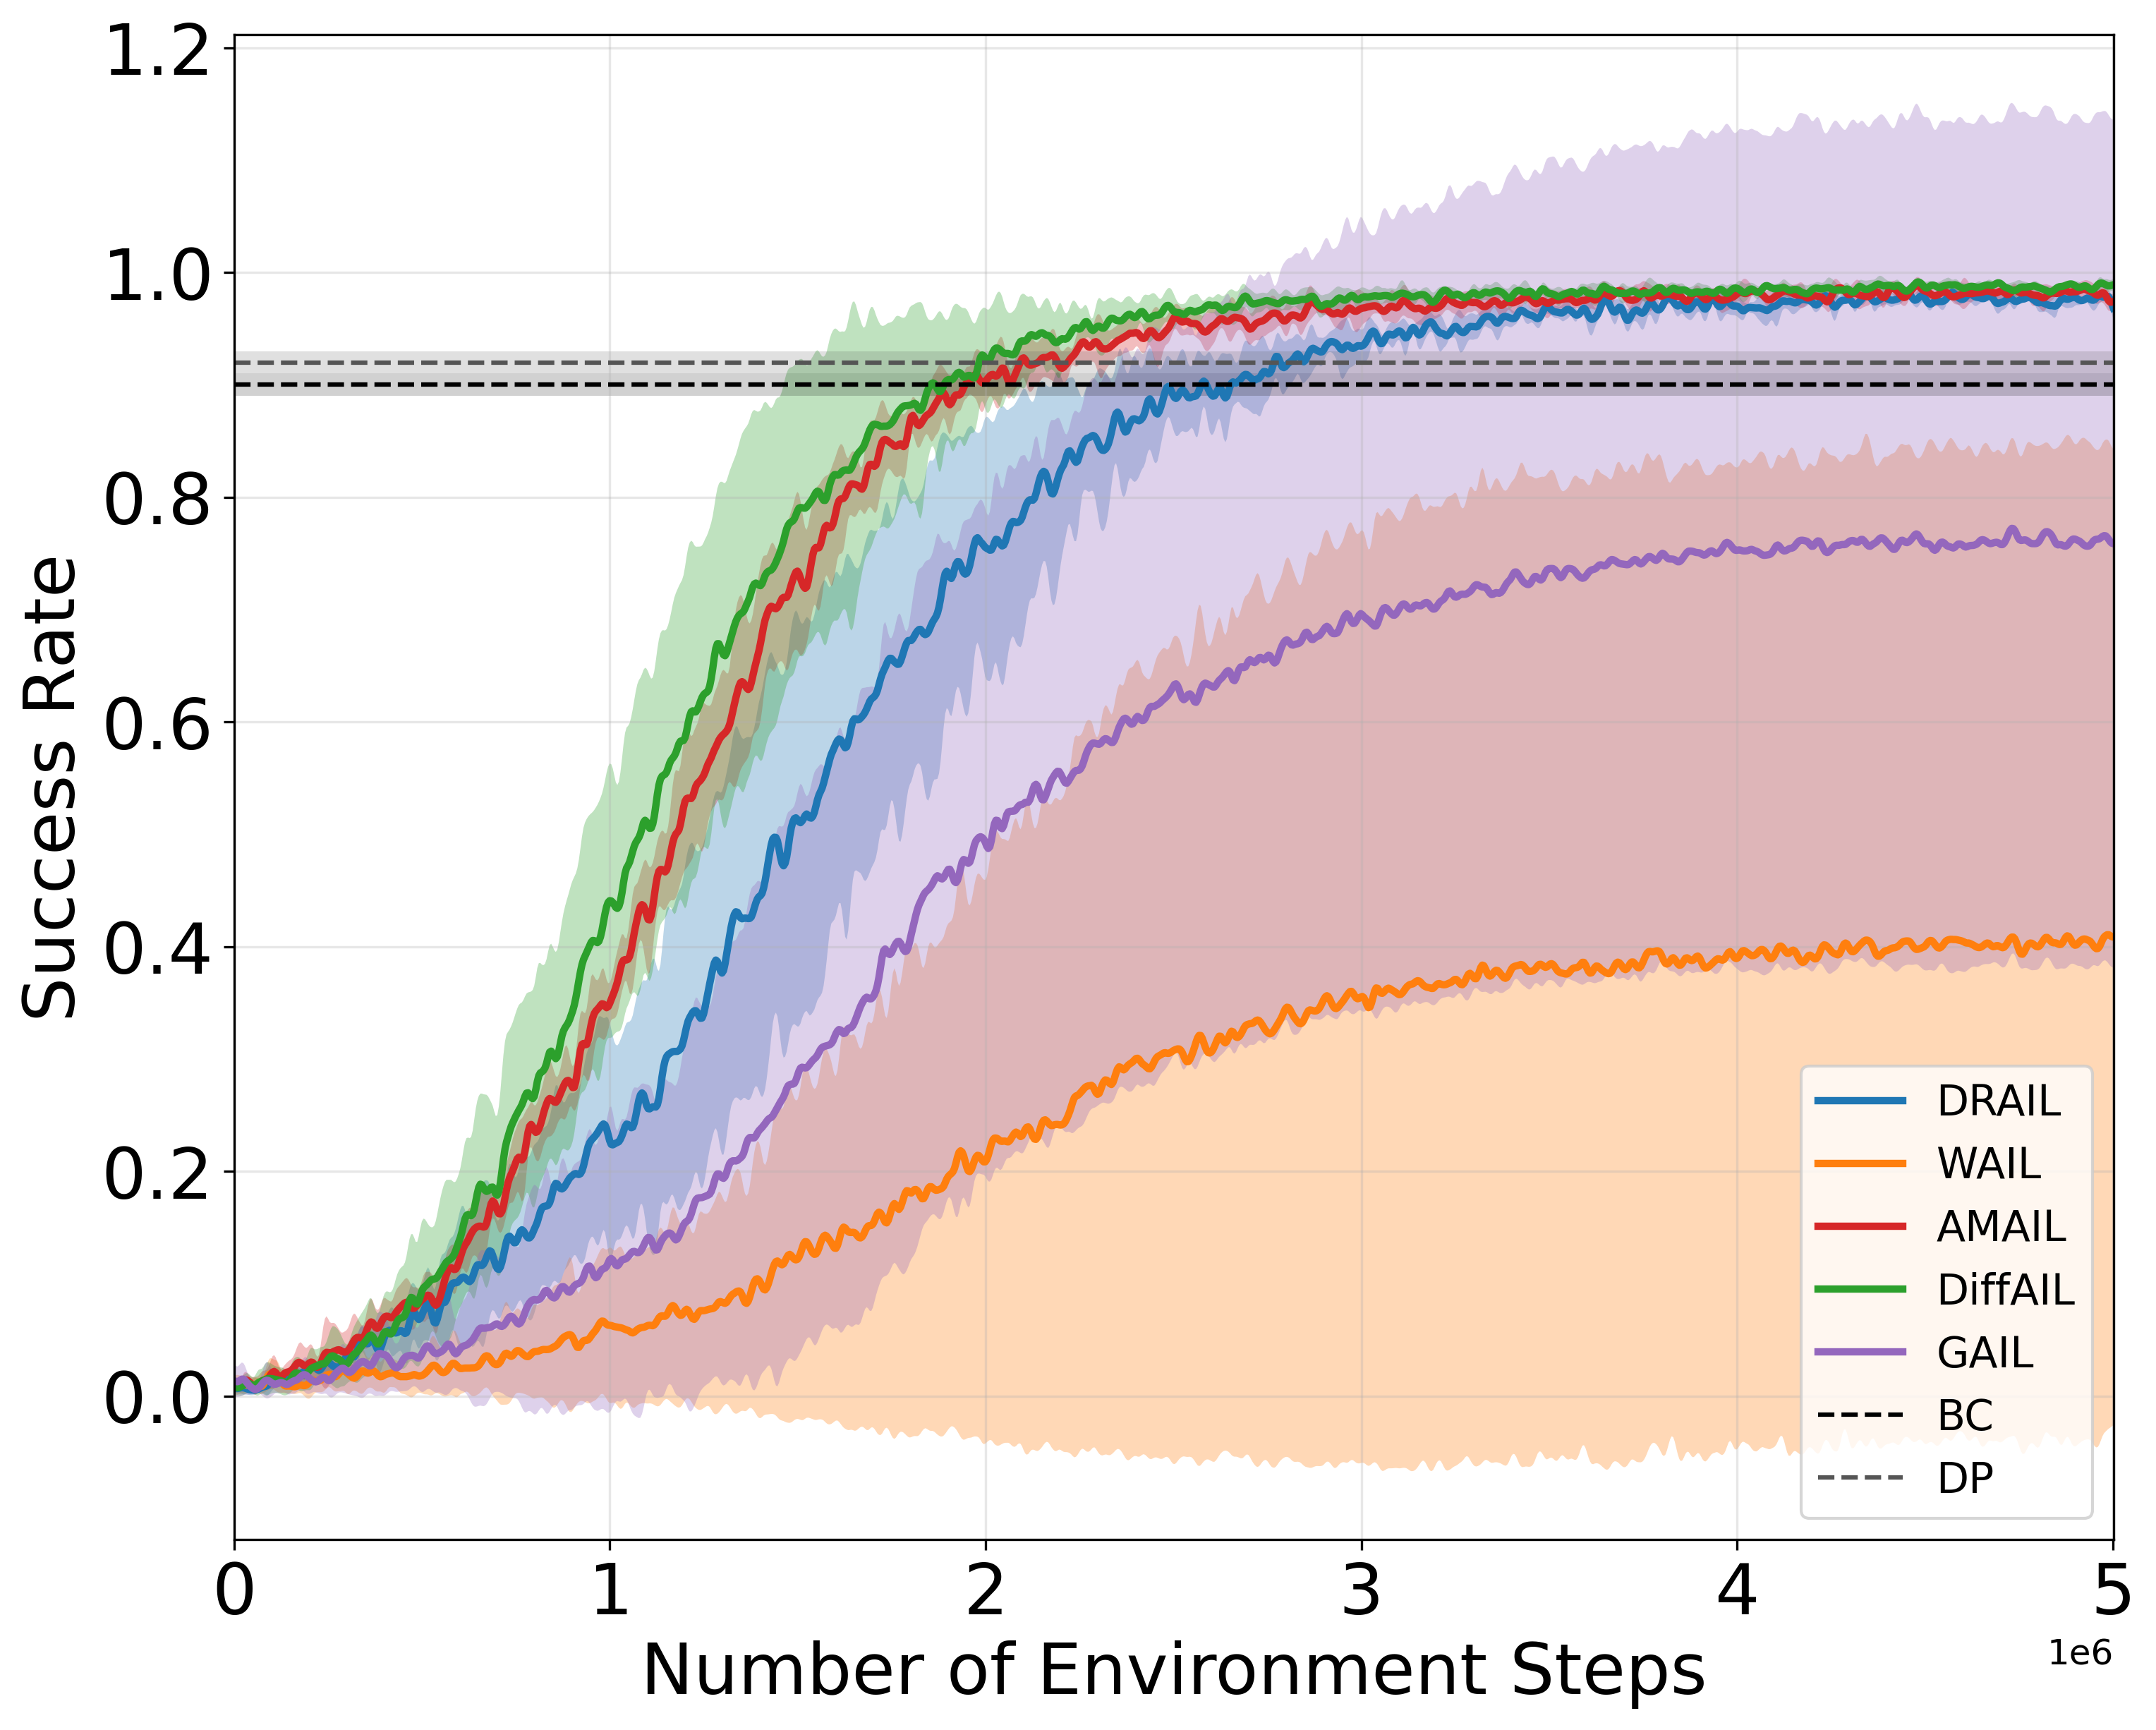
\includegraphics[width=0.33\textwidth]{Hand.png}%
\label{Hand}}%
\hfill
\subfloat[MAZE]{%
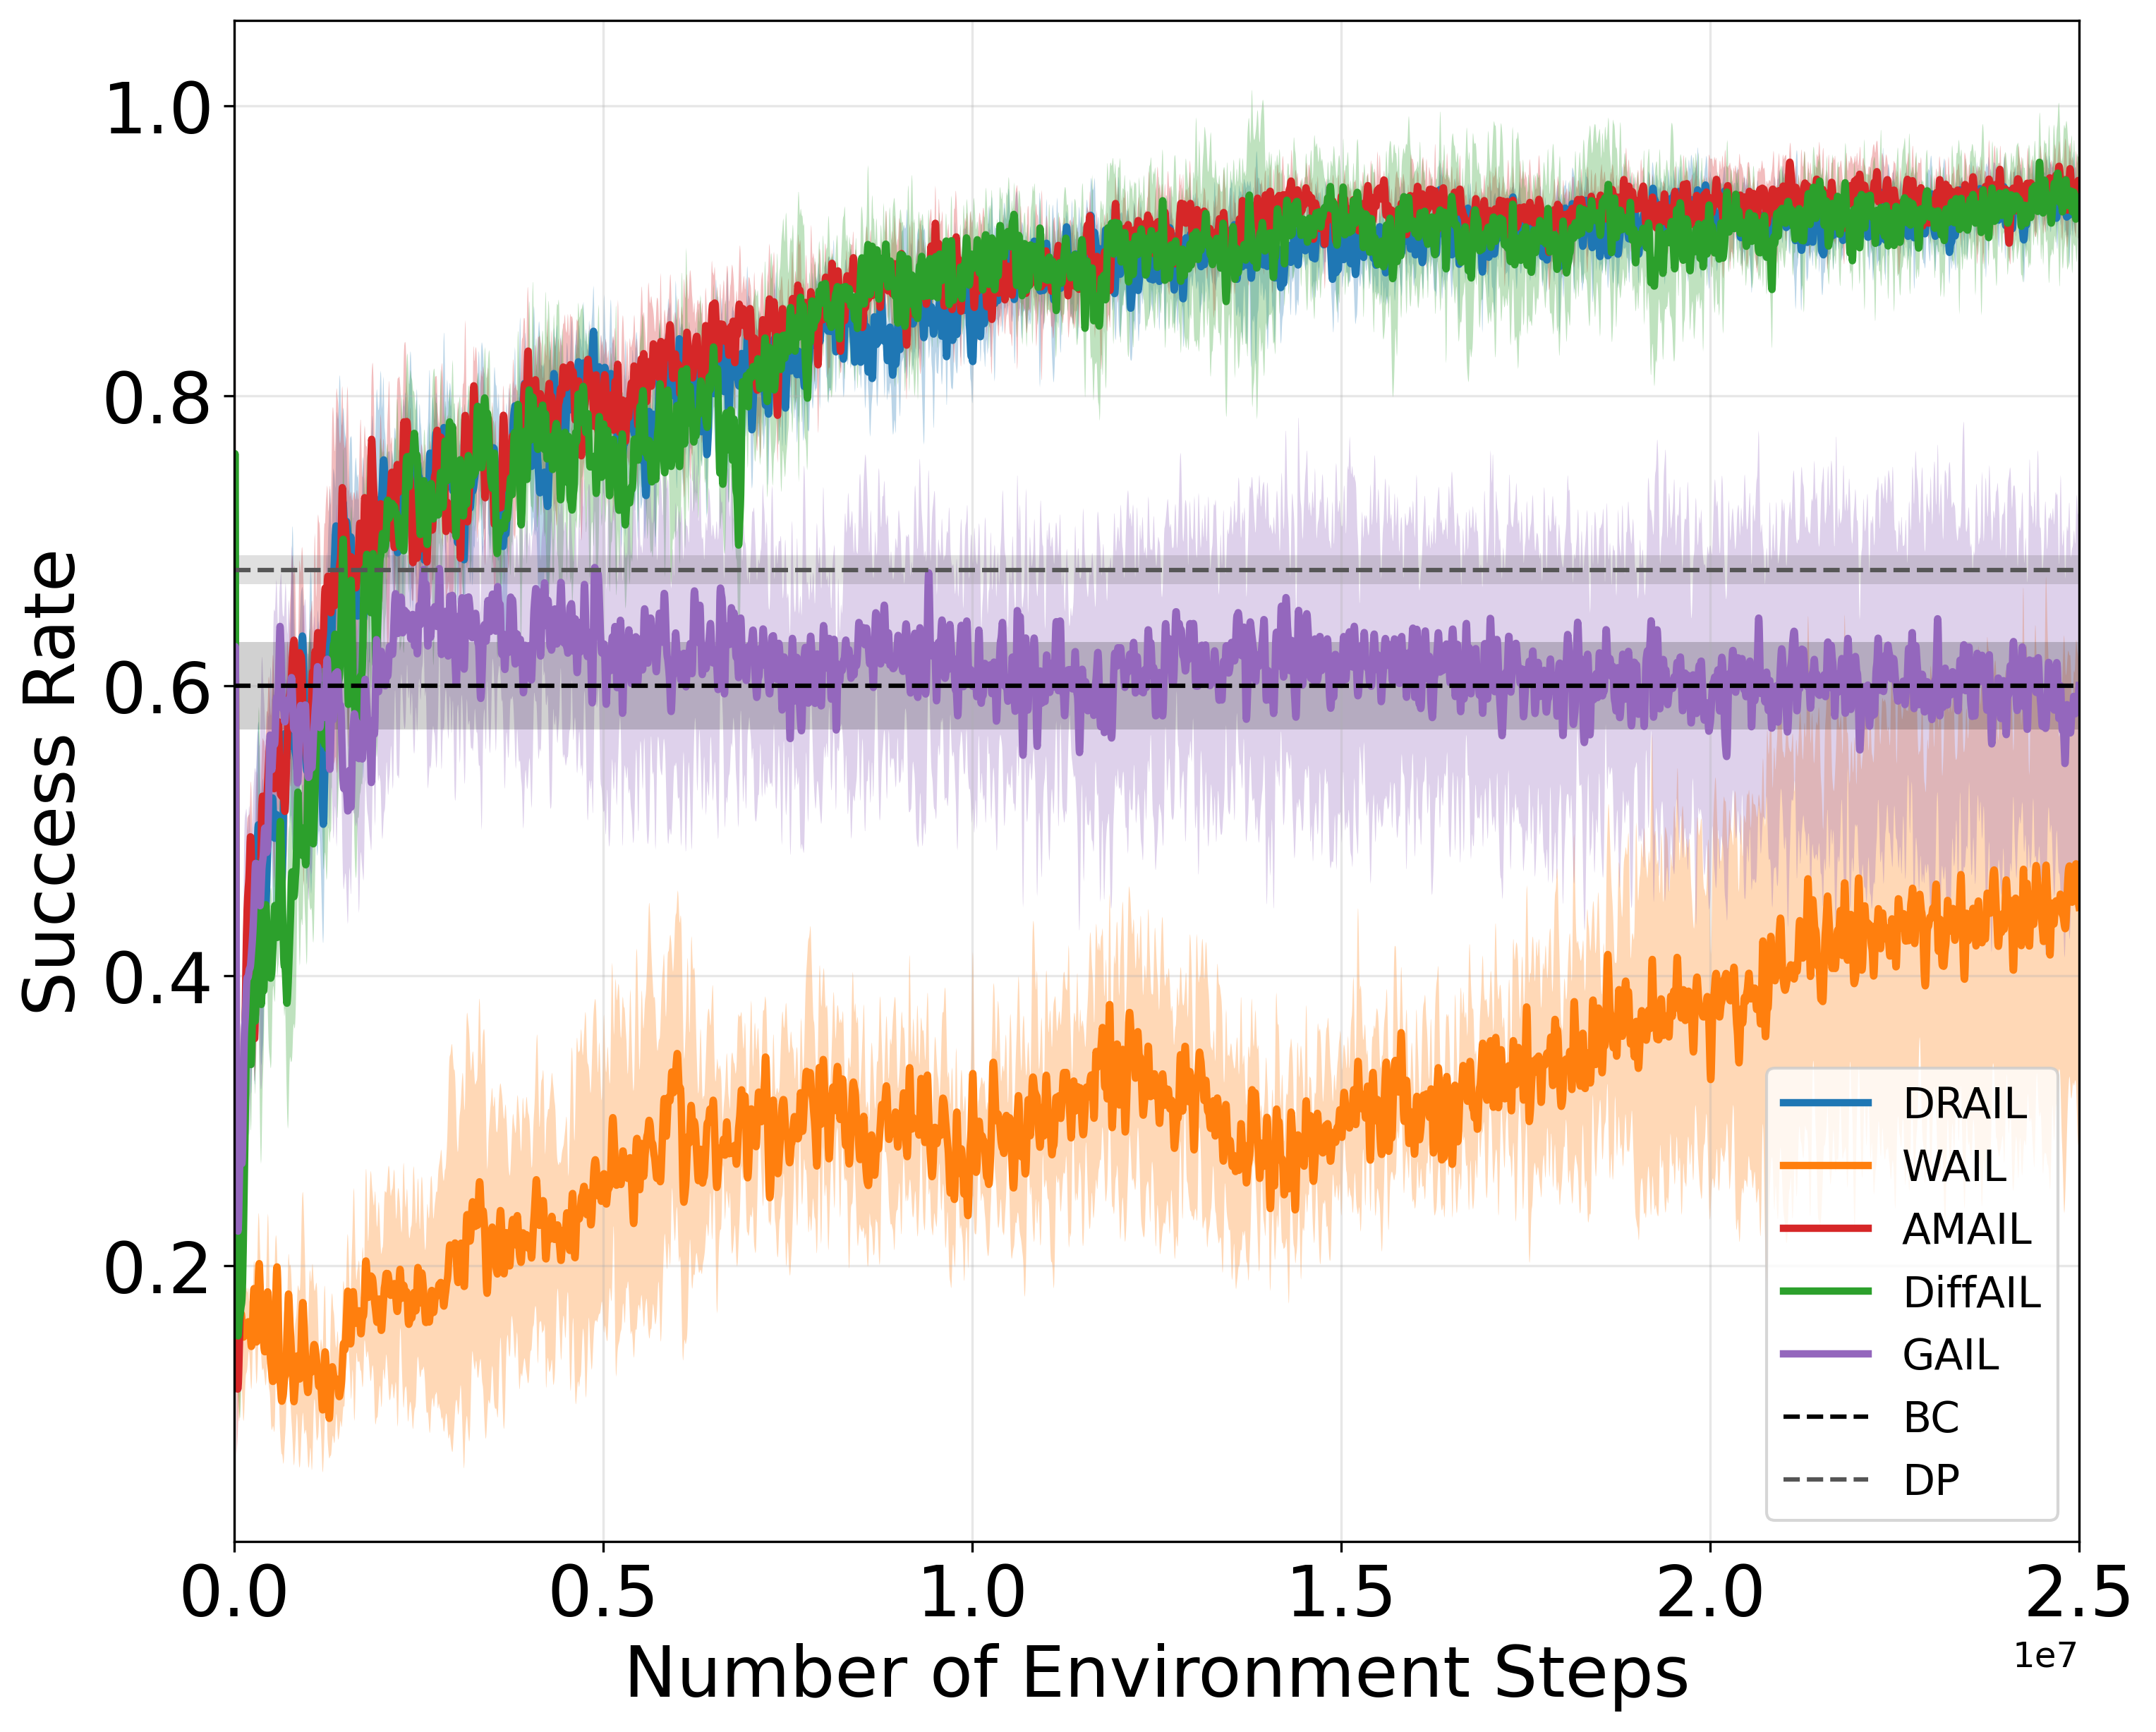
\includegraphics[width=0.33\textwidth]{Maze.png}%
\label{Maze}}%
\hfill
\subfloat[WALKER]{%
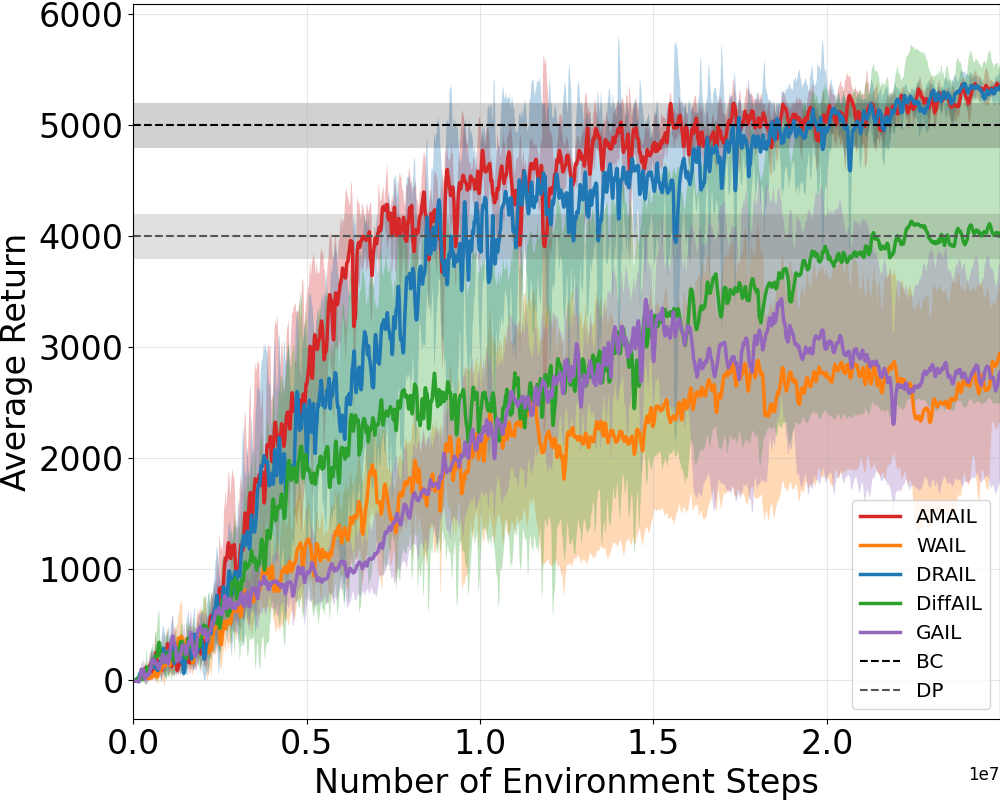
\includegraphics[width=0.33\textwidth]{Walker.png}%
\label{Walker}}%

\caption{\textbf{Learning efficiency}. Our method is compared against six baseline methods across six environments, with each experiment repeated over five random seeds; the curves report mean performance and the shaded regions indicate pointwise standard deviation. Across all tasks and training stages, AMAIL demonstrates faster convergence, reduced variance, and consistently superior performance relative to competing approaches.}
\label{fig_sim2}
\end{figure*}

\subsection{Baselines}
To validate the effectiveness of the proposed framework, comparisons are conducted with representative imitation learning and adversarial learning methods.

\textbf{$\bullet$ Behavior Cloning (BC)}\cite{torabi2018behavioral} is a supervised imitation learning method that directly learns a deterministic or stochastic mapping from states to actions using expert demonstrations. As one of the most fundamental imitation learning approaches, BC serves as a lower-bound baseline, particularly sensitive to covariate shift due to the absence of environment interaction during training.

\textbf{$\bullet$ Diffusion Policy (DP)}\cite{chi2025diffusion,pearce2023imitating,reuss2023goal} models the target policy as a conditional diffusion process. Given a state input and sampled Gaussian noise, the model iteratively denoises the action representation to generate control outputs. As an offline generative policy learning approach, DP is capable of modeling complex, multimodal action distributions.

\textbf{$\bullet$ Generative Adversarial Imitation Learning (GAIL)}\cite{ho2016generative} formulates imitation learning as a minimax game between a policy generator and a discriminator. The discriminator distinguishes expert trajectories from policy-generated trajectories, while the policy is trained to match the expert's occupancy measure. This framework enables indirect reward learning through adversarial optimization.

\textbf{$\bullet$ Wasserstein Adversarial Imitation Learning (WAIL)}\cite{xiao2019wasserstein} replaces the Jensen-Shannon divergence in GAIL with the Wasserstein distance, leading to smoother gradient signals and improved training stability. By leveraging optimal transport principles, WAIL mitigates reward oscillation and gradient vanishing issues observed in standard adversarial imitation learning.

\textbf{$\bullet$ Diffusion Adversarial Imitation Learning (DiffAIL)}\cite{wang2024diffail} incorporates a diffusion model into the adversarial imitation learning framework. The diffusion loss is integrated into the discriminator's objective, enabling more accurate modeling of the expert data distribution. This enhances the discriminator's capacity to capture complex and high-dimensional action patterns.

\textbf{$\bullet$ Diffusion Rewards Adversarial Imitation Learning (DRAIL)}\cite{lai2024diffusion} integrates diffusion-based modeling into the reward learning component of GAIL. By using diffusion processes to characterize the similarity between current states and target states, DRAIL generates smoother and more informative reward signals, thereby alleviating instability commonly observed in adversarial training.



\begin{table*}[!t]
\centering
\caption{Performance Comparison Across Six Tasks}
\label{tab:cluster_tnnls}

\setlength{\tabcolsep}{5pt}
\renewcommand{\arraystretch}{1.1}

\resizebox{\textwidth}{!}{%
\begin{tabular}{
lccccccc
}
\toprule
\multirow{2}{*}{\textbf{Task}} 
& \multicolumn{3}{c}{\textbf{Representative algorithms of imitation learning}} 
& \multicolumn{4}{c}{\textbf{Novel algorithms based on adversarial imitation learning}} \\
\cmidrule(lr){2-4}
\cmidrule(lr){5-8}
& \textbf{BC} & \textbf{DP} & \textbf{GAIL} & \textbf{WAIL} & \textbf{DiffAIL} & \textbf{DRAIL} & \textbf{AMAIL} \\
\midrule

FETCHPUSH & $81.00\%\pm 2.10\%$ & $89.00\%\pm 1.01 \%$ & $85.13\% \pm 17.00\%$ & $62.22\% \pm 45.70\%$ & $98.12\%\pm 0.48\%$ & $97.90\%\pm 0.53\%$ & \textbf{98.16\% $\pm$ 0.19\%} \\

FETCHPICK & $41.01\%\pm 5.10\%$ & $70.12\%\pm 3.23\%$ & $1.01\%\pm 0.07\%$ & $1.10\%\pm 0.10\%$ & $39.38\%\pm 48.24\%$ & \textbf{98.96\%$\pm$ 0.72\%}  & $98.90\% \pm 0.71\%$ \\

ANTREACH & $55.12\% \pm 2.10\%$ & \textbf{57.78\% $\pm$ 1.01\%} & $11.02\%\pm 7.35\%$ & $23.58\%\pm 15.66\%$ & $37.92\%\pm 3.47\%$ & $49.80\% \pm 2.79\%$ & $50.04\%\pm 1.37\%$ \\

HANDROTATE & $89.93\% \pm 1.09\%$ & $91.14\% \pm 1.24\%$ & $76.26\%\pm 37.74\%$ & $40.72\%\pm 43.84\%$ & \textbf{98.88\%$\pm$ 0.44\%} & $97.42\%\pm 0.74\%$ & $97.82\%\pm 0.34\%$ \\

MAZE & $60.02\% \pm 1.21\%$& $68.31\%\pm 4.10\%$ & $59.54\%\pm 12.42\%$ & $44.96\%\pm 16.07\%$ & $93.58\%\pm 3.36\%$ & $94.42\%\pm 1.50\%$ & \textbf{94.72\% $\pm$ 1.19\%} \\

WALKER & $4023.75\pm 476.12$& $5003.13\pm 549.26$& $2766.46\pm 990.35$ & $2938.65\pm 616.98$ & $4015.13\pm 1522.03$ & $5344.14\pm 68.99$ & \textbf{5354.22 $\pm$ 50.87} \\

\bottomrule
\end{tabular}
}
\end{table*}

\begin{figure*}[!t]
\centering

\subfloat[FETCHPUSH]{%
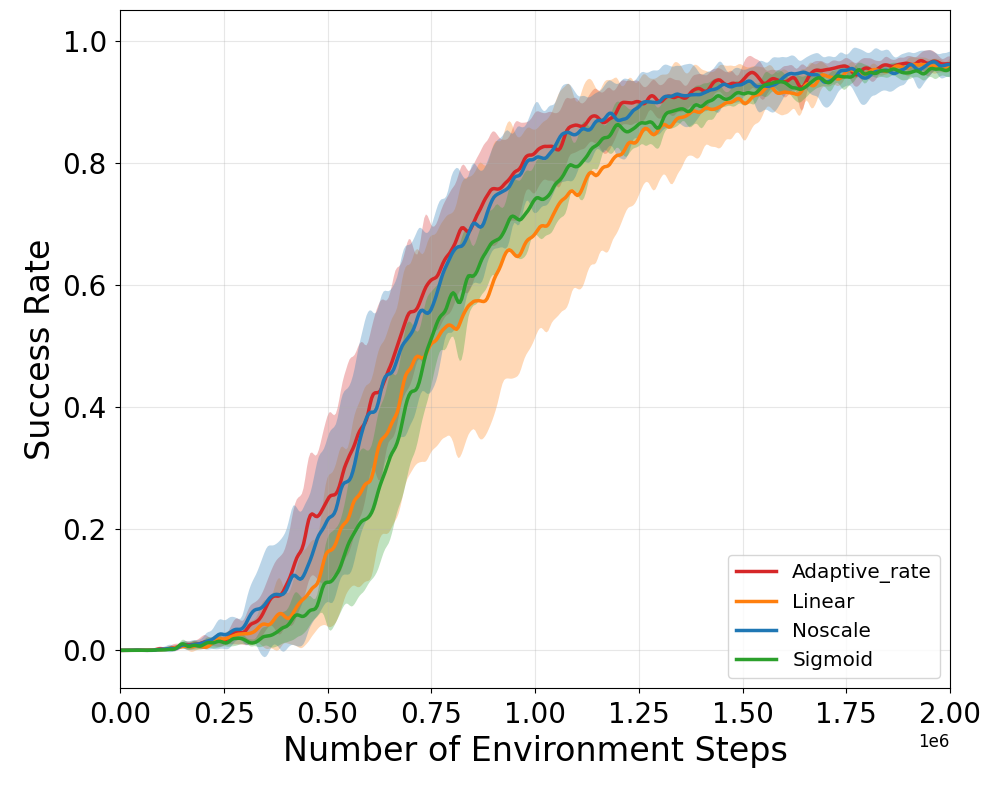
\includegraphics[width=0.33\textwidth]{learning_rate.png}%
\label{The training effects with different weights}}%
\hspace{0.02\textwidth}
\subfloat[Rate]{%
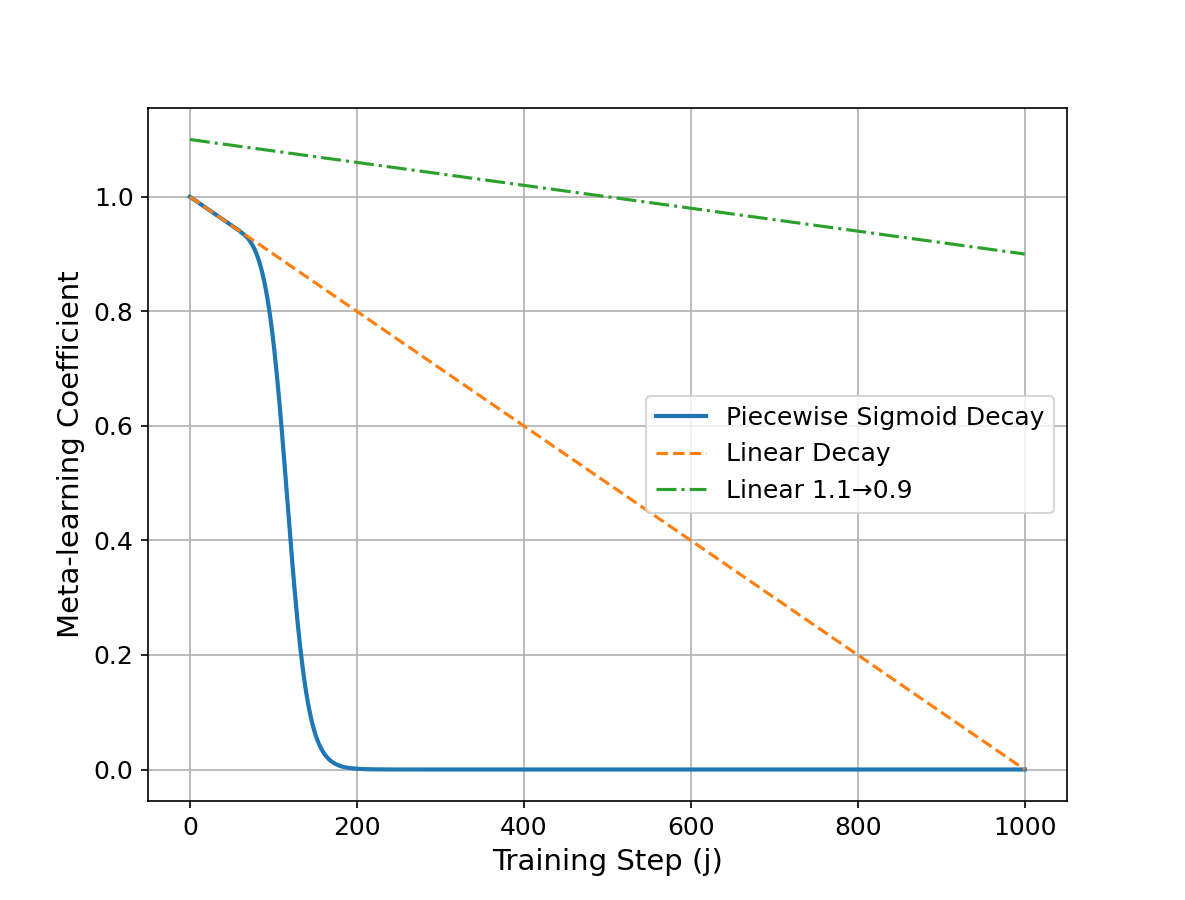
\includegraphics[width=0.38\textwidth]{rate.png}%
\label{rate}}%


\caption{\textbf{Meta-learning Network Coefficient}. The parameters of the linear and sigmoid decay schedules were tuned to their optimal values and evaluated in FetchPush under 2.0$\times$ noise. Results indicate that dynamic weighting outperforms both linear and sigmoid strategies. Output scaling further enhances performance, especially when there is a large magnitude gap between the meta-learning outputs and the reinforcement learning objective.}
\label{fig_sim3}
\end{figure*}

\subsection{Results and Analysis}
To ensure a systematic and fair evaluation,  all methods are trained using identical datasets and evaluated across six benchmark tasks. Each experiment is repeated over five random seeds, and both mean performance and standard deviation are reported to assess effectiveness and stability.
It is worth noting that behavior cloning (BC) and diffusion policy are purely offline approaches and therefore do not interact with the environment during training. For comparability, their success rates are plotted as horizontal reference lines in the performance curves.

We first examine learning efficiency under standard expert settings.
All models were trained using the complete expert dataset with identical noise conditions (1$\times$, consistent with the expert data collection process). Under these controlled settings, our method achieves performance comparable to or exceeding existing algorithms across all tasks, and demonstrates clear advantages in several environments. In particular, AMAIL improves expert data utilization through adaptive meta-guided optimization. On the FETCHPUSH, FETCHPICK, HANDROTATE, and WALKER tasks, it rapidly converges to expert-level performance, indicating that the adaptive meta-learning network (AMLN) effectively captures the latent behavioral structure of expert demonstrations and provides meaningful guidance to the policy network. Conventional adversarial methods such as GAIL and WAIL exhibit severe instability in high-dimensional sparse-reward manipulation tasks, leading to poor convergence in FETCHPICK. Moreover, performance variance across random seeds is reduced, suggesting that the adaptive learning mechanism enhances robustness to noise and improves generalization. By adopting a two-layer adaptive meta-learning architecture, AMAIL extracts high-level structural information from offline demonstrations and transforms it into auxiliary guidance rewards. Unlike conventional imitation learning methods that focus solely on behavior matching, AMAIL models the intrinsic decision logic underlying expert behavior and leverages it to shape policy optimization.

To further investigate the role of meta-guidance, we analyze how to regulate the intervention ratio of the adaptive meta-learning network (AMLN) during training. Intuitively, stronger intervention is desirable in the early stages to accelerate representation alignment, while a gradual reduction is beneficial later to avoid over-regularization and performance degradation. In imitation learning, inappropriate intervention can destabilize training or suppress policy improvement. To address this, we use the diffusion discriminator's output to estimate demonstration confidence and dynamically adjust the influence of the adaptive meta-learning network on policy updates. We compare this adaptive mechanism with commonly used linear decay and sigmoid decay schedules in the FetchPush environment. Because the magnitude of the adaptive meta-guided optimization outputs may differ from reinforcement learning signals, direct combination can lead to under- or over-dominance. Therefore, we rescale the weighted adaptive meta-guided optimization outputs to ensure compatibility across tasks and maintain balanced optimization dynamics.

This adaptive control mechanism provides two complementary benefits. First, it encourages efficient exploration by emphasizing high-value behavioral patterns distilled from expert data. Second, it suppresses misleading updates caused by low-confidence or noisy demonstrations. As a result, AMAIL achieves higher data efficiency and stronger robustness, particularly in scenarios with limited or imperfect expert demonstrations.

\begin{figure*}[!t]
\centering

\subfloat[Noise $\times1.25$]{%
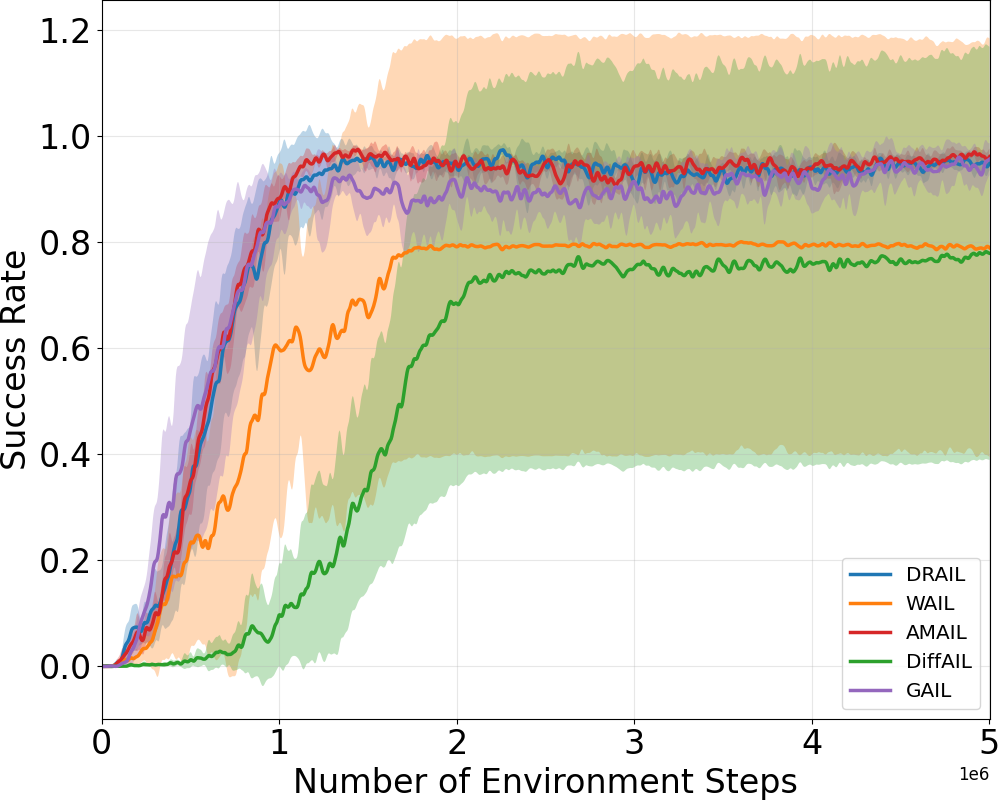
\includegraphics[width=0.33\textwidth]{1.25.png}%
\label{FETCHPUSH 1.25}}%
\hfill
\subfloat[Noise $\times1.75$]{%
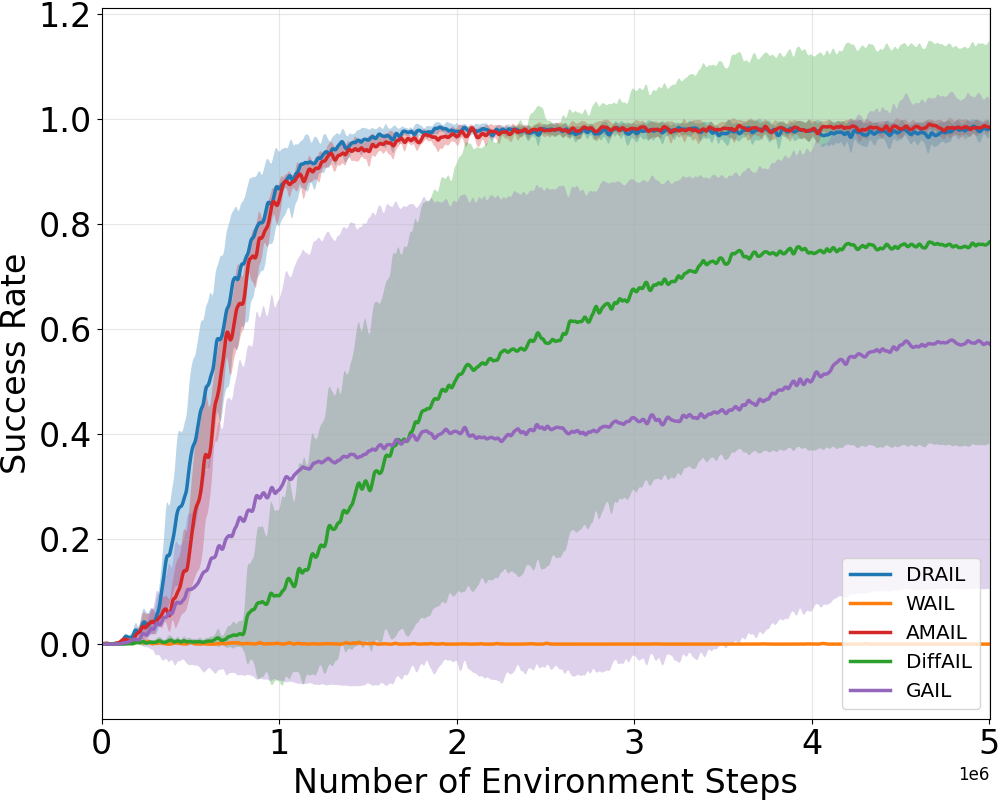
\includegraphics[width=0.33\textwidth]{1.75.png}%
\label{FETCHPUSH x1.75}}%
\hfill
\subfloat[Noise $\times2.00$]{%
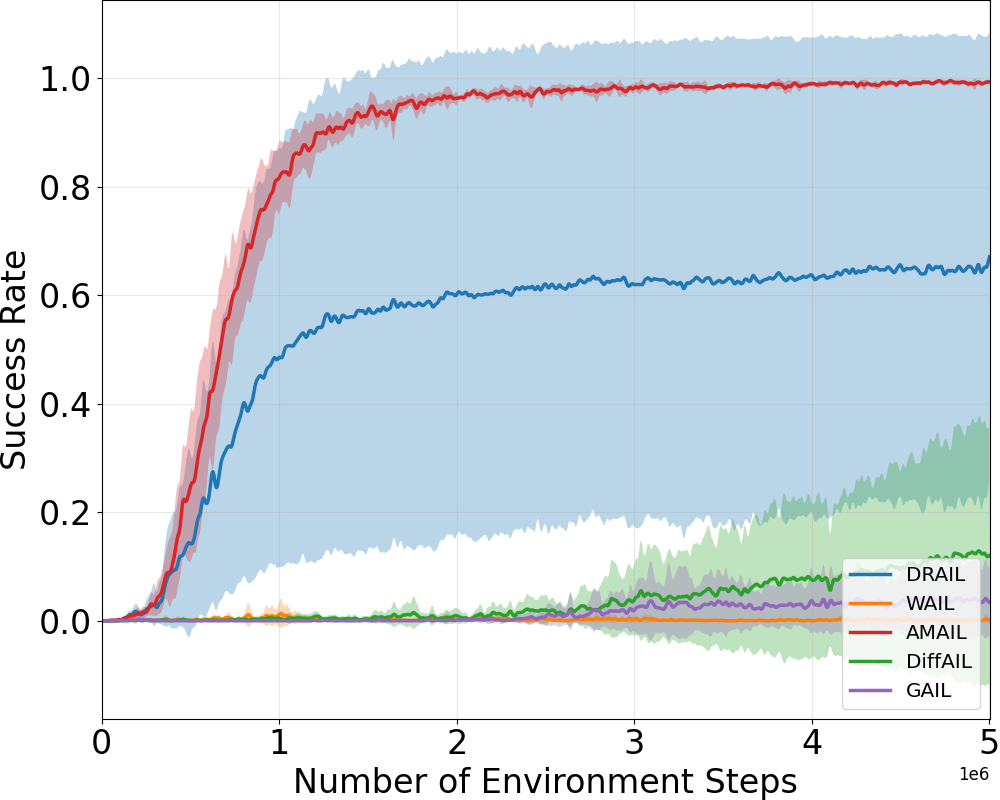
\includegraphics[width=0.33\textwidth]{2.00.png}%
\label{FETCHPUSH x2.00}}%


\caption{\textbf{Noise resistance and generalization ability}. Performance comparison on FETCHPUSH under noise intensities of $\times1.25$, $\times1.75$, and $\times2.00$; curves show mean success rate over five random seeds and shaded regions indicate standard deviation. AMAIL maintains stable convergence and superior final performance as noise increases, demonstrating strong robustness against corrupted expert demonstrations.}
\label{fig_sim4}
\end{figure*}

To further evaluate the robustness and generalization benefits introduced by the adaptive weighting mechanism, we conducted additional experiments on the complete FETCHPUSH dataset under progressively increasing noise levels. Specifically, Gaussian noise was injected into both the initial states and target states of the demonstrations with intensities of 1.25$\times$, 1.75$\times$, and 2.0$\times$ relative to the original data collection setting. This setup simulates blurred or corrupted expert trajectories and forces the models to extract informative behavioral signals from ambiguous state distributions.

As the noise level increased, conventional imitation and adversarial methods suffered significant performance degradation, often accompanied by unstable convergence. Diffusion-based baselines such as DRAIL and DiffAIL demonstrated relatively stronger tolerance to moderate noise due to their generative modeling capability. However, in high-noise regimes, they exhibited slower convergence and eventual performance collapse, primarily because noisy demonstrations weakened the reliability of the learned distributional guidance.

In contrast, AMAIL maintained stable training dynamics and showed minimal degradation in both convergence speed and final performance as noise intensity increased. This robustness stems from the adaptive confidence weighting mechanism, which effectively suppresses the influence of corrupted samples and mitigates systematic bias in the adaptive meta-learning network (AMLN) under high-noise conditions. As a result, AMAIL preserves reliable policy improvement even when expert information is substantially perturbed, demonstrating improved robustness against noisy demonstrations.



\section{Conclusion}
In this paper, a noise-robust adaptive meta-adversarial imitation learning approach has been proposed, which integrates an adaptive meta-learning architecture with a diffusion-based discriminator to improve imitation learning performance.
An adaptive meta-learning network has been designed to capture the underlying optimization structure embedded in expert trajectories, which enables efficient and stable policy adaptation. In addition, an adaptive weighting mechanism has been introduced to regulate the influence of adaptive meta-guided optimization updates based on diffusion loss, thereby suppressing low-confidence samples and improving robustness under distributional perturbations.
Experimental results on MuJoCo and PyBullet benchmarks have demonstrated that the proposed method achieves superior learning efficiency, convergence stability, and robustness compared with representative baseline methods. 


Future work will focus on extending the proposed framework to high-dimensional observation spaces, such as visual inputs. Integrating the adaptive meta-learning mechanism with large-scale perception models may enable efficient processing of image-based data. In addition, the data-efficient learning capability of the framework can be further explored for adapting pretrained policies to downstream tasks, which provides a promising direction for robust and data-efficient policy adaptation in real-world robotic systems.

\bibliographystyle{IEEEtran}
\bibliography{IEEEbib}
% \begin{thebibliography}{1}




% \bibitem{ref2}
% B. D. Argall, S. Chernova, M. Veloso, and B. Browning, “A survey of robot learning from demonstration,” {\it{Robotics and Autonomous Systems}}, vol. 57, no. 5, pp. 469-483, May 2009, doi: 10.1016/j.robot.2008.10.024.


% \bibitem{ref3}
% F. Codevilla, M. Müller, A. López, V. Koltun, and A. Dosovitskiy, “End-to-End Driving Via Conditional Imitation Learning,” in {\it{2018 IEEE International Conference on Robotics and Automation (ICRA)}}, May 2018, pp. 4693-4700. doi: 10.1109/ICRA.2018.8460487.


% \bibitem{ref4}
% D. Silver et al., “Mastering the game of Go with deep neural networks and tree search,” {\it{Nature}}, vol. 529, no. 7587, pp. 484-489, Jan. 2016, doi: 10.1038/nature16961.


% \bibitem{ho2016generative}J. Ho and S. Ermon, “Generative Adversarial Imitation Learning,” in {\it{Advances in Neural Information Processing Systems}}, Curran Associates, Inc., 2016. Accessed: May 06, 2026. [Online]. Available: \url{https://proceedings.neurips.cc/paper_files/paper/2016/hash/cc7e2b878868cbae992d1fb743995d8f-Abstract.html}




% \bibitem{ref6}
% M. Arjovsky and L. Bottou, “Towards Principled Methods for Training Generative Adversarial Networks,” presented at {\it{the International Conference on Learning Representations}}, Feb. 2017. Accessed: Apr. 29, 2026. [Online]. Available: \url{https://openreview.net/forum?id=Hk4_qw5xe}


% \bibitem{ref7}
% C. Finn, S. Levine, and P. Abbeel, “Guided cost learning: deep inverse optimal control via policy optimization,” in {\it{Proceedings of the 33rd International Conference on International Conference on Machine Learning}} - Volume 48, in ICML'16. New York, NY, USA: JMLR.org, Jun. 2016, pp. 49-58.


% \bibitem{ding2019goal}
% Y. Ding, C. Florensa, P. Abbeel, and M. Phielipp, “Goal-conditioned Imitation Learning,” in {\it{Advances in Neural Information Processing Systems}}, Curran Associates, Inc., 2019. Accessed: Apr. 29, 2026. [Online]. Available: \url{https://proceedings.neurips.cc/paper_files/paper/2019/hash/c8d3a760ebab631565f8509d84b3b3f1-Abstract.html}


% \bibitem{torabi2018generative}
% F. Torabi, G. Warnell, and P. Stone, “Generative Adversarial Imitation from Observation,” in {\it{Proceedings of the 36th International Conference on Machine Learning}}, in ICML'19. New York, NY, USA: JMLR.org, Jun. 2019, pp. 4692-4701.


% \bibitem{wang2024diffail}
% B. Wang, G. Wu, T. Pang, Y. Zhang, and Y. Yin, “DiffAIL: Diffusion Adversarial Imitation Learning,” {\it{Proceedings of the AAAI Conference on Artificial Intelligence}}, vol. 38, no. 14, pp. 15447-15455, Mar. 2024, doi: 10.1609/aaai.v38i14.29470.


% \bibitem{fu2017learning}
% J. Fu, K. Luo, and S. Levine, “Learning Robust Rewards with Adverserial Inverse Reinforcement Learning,” presented at {\it{the International Conference on Learning Representations}}, Feb. 2018. Accessed: May 05, 2026. [Online]. Available: \url{https://openreview.net/forum?id=rkHywl-A-}


% \bibitem{RB-GAIL}
% Z. Shi, X. Zhang, Y. Fang, C. Li, G. Liu, and J. Zhao, “Ranking-Based Generative Adversarial Imitation Learning,” {\it{IEEE Robotics and Automation Letters}}, pp. 1-8, 2024, doi: 10.1109/LRA.2024.3451360.


% \bibitem{kostrikov2019imitation}
% I. Kostrikov, O. Nachum, and J. Tompson, “Imitation Learning via Off-Policy Distribution Matching,” presented at {\it{the International Conference on Learning Representations}}, Sep. 2019. Accessed: Jan. 08, 2026. [Online]. Available: \url{https://openreview.net/forum?id=Hyg-JC4FDr}




% \bibitem{kim2021demodice}
% G.-H. Kim et al., “DemoDICE: Offline Imitation Learning with Supplementary Imperfect Demonstrations,” presented at the {\it{International Conference on Learning Representations}}, Oct. 2021. Accessed: Dec. 13, 2025. [Online]. Available: \url{https://openreview.net/forum?id=BrPdX1bDZkQ}


% \bibitem{garg2021iq}
% D. Garg, S. Chakraborty, C. Cundy, J. Song, and S. Ermon, “IQ-Learn: Inverse soft-Q Learning for Imitation,” in {\it{Advances in Neural Information Processing Systems}}, Curran Associates, Inc., 2021, pp. 4028-4039. Accessed: May 05, 2026. [Online]. Available: \url{https://proceedings.neurips.cc/paper/2021/hash/210f760a89db30aa72ca258a3483cc7f-Abstract.html}



% \bibitem{reddy2019sqil}
% S. Reddy, A. D. Dragan, and S. Levine, “SQIL: Imitation Learning via Reinforcement Learning with Sparse Rewards,” presented at {\it{the International Conference on Learning Representations}}, Sep. 2019. Accessed: Jan. 08, 2026. [Online]. Available: \url{https://openreview.net/forum?id=S1xKd24twB}


% \bibitem{wu2019imitation}
% Y.-H. Wu, N. Charoenphakdee, H. Bao, V. Tangkaratt, and M. Sugiyama, “Imitation Learning from Imperfect Demonstration,” in {\it{Proceedings of the 36th International Conference on Machine Learning}}, PMLR, May 2019, pp. 6818-6827. Accessed: May 05, 2026. [Online]. Available: \url{https://proceedings.mlr.press/v97/wu19a.html}




% \bibitem{wang2021learning}
% Y. Wang, C. Xu, B. Du, and H. Lee, “Learning to Weight Imperfect Demonstrations,” in {\it{Proceedings of the 38th International Conference on Machine Learning}}, PMLR, Jul. 2021, pp. 10961-10970. Accessed: May 05, 2026. [Online]. Available: \url{https://proceedings.mlr.press/v139/wang21aa.html}


% \bibitem{chi2025diffusion}
% C. Chi et al., “Diffusion policy: Visuomotor policy learning via action diffusion,” {\it{The International Journal of Robotics Research}}, vol. 44, no. 10-11, pp. 1684-1704, Sep. 2025, doi: 10.1177/02783649241273668.



% \bibitem{pearce2023imitating}
% T. Pearce et al., “Imitating Human Behaviour with Diffusion Models,” presented at {\it{the The Eleventh International Conference on Learning Representations}}, Sep. 2022. Accessed: May 06, 2026. [Online]. Available: https://openreview.net/forum?id=Pv1GPQzRrC8




% \bibitem{yuan2019adversarial}
% X. Yuan, P. He, Q. Zhu, and X. Li, “Adversarial Examples: Attacks and Defenses for Deep Learning,” {\it{IEEE Transactions on Neural Networks and Learning Systems}}, vol. 30, no. 9, pp. 2805-2824, Sep. 2019, doi: 10.1109/TNNLS.2018.2886017.




% \bibitem{song2022learning}
% H. Song, M. Kim, D. Park, Y. Shin, and J.-G. Lee, “Learning From Noisy Labels With Deep Neural Networks: A Survey,” {\it{IEEE Transactions on Neural Networks and Learning Systems}}, vol. 34, no. 11, pp. 8135-8153, Nov. 2023, doi: 10.1109/TNNLS.2022.3152527.



% \bibitem{li2022backdoor}
% Y. Li, Y. Jiang, Z. Li, and S.-T. Xia, “Backdoor Learning: A Survey,” {\it{IEEE Transactions on Neural Networks and Learning Systems}}, vol. 35, no. 1, pp. 5-22, Jan. 2024, doi: 10.1109/TNNLS.2022.3182979.


% \bibitem{DRAIL}
% C.-M. Lai, H.-C. Wang, P.-C. Hsieh, Y.-C. F. Wang, M.-H. Chen, and S.-H. Sun, “Diffusion-Reward Adversarial Imitation Learning,” {\it{Advances in Neural Information Processing Systems}}, vol. 37, pp. 95456-95487, Dec. 2024, doi: 10.52202/079017-3025.

% \bibitem{MAML}
% C. Finn, P. Abbeel, and S. Levine, “Model-Agnostic Meta-Learning for Fast Adaptation of Deep Networks,” in {\it{Proceedings of the 34th International Conference on Machine Learning}} - Volume 70, in ICML'17. New York, NY, USA: JMLR.org, Aug. 2017, pp. 1126-1135.


% \bibitem{Denoising Diffusion Probabilistic Models}
% J. Ho, A. Jain, and P. Abbeel, “Denoising Diffusion Probabilistic Models,” in {\it{Advances in Neural Information Processing Systems, Curran Associates}}, Inc., 2020, pp. 6840-6851. Accessed: May 06, 2026. [Online]. Available: \url{https://proceedings.neurips.cc/paper/2020/hash/4c5bcfec8584af0d967f1ab10179ca4b-Abstract.html}



% \end{thebibliography}


\newpage

% \section{Biography Section}
% If you have an EPS/PDF photo (graphicx package needed), extra braces are
%  needed around the contents of the optional argument to biography to prevent
%  the LaTeX parser from getting confused when it sees the complicated
%  $\backslash${\tt{includegraphics}} command within an optional argument. (You can create
%  your own custom macro containing the $\backslash${\tt{includegraphics}} command to make things
%  simpler here.)
 
% \vspace{11pt}

% \bf{If you include a photo:}\vspace{-33pt}
% \begin{IEEEbiography}[{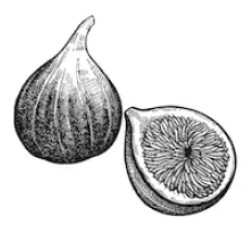
\includegraphics[width=1in,height=1.25in,clip,keepaspectratio]{fig1}}]{Michael Shell}
% Use $\backslash${\tt{begin\{IEEEbiography\}}} and then for the 1st argument use $\backslash${\tt{includegraphics}} to declare and link the author photo.
% Use the author name as the 3rd argument followed by the biography text.
% \end{IEEEbiography}

% \vspace{11pt}

% \bf{If you will not include a photo:}\vspace{-33pt}
% \begin{IEEEbiographynophoto}{John Doe}
% Use $\backslash${\tt{begin\{IEEEbiographynophoto\}}} and the author name as the argument followed by the biography text.
% \end{IEEEbiographynophoto}




\vfill

\end{document}


